% =====================================================================
% AAAI-27 submission — formatted to the AAAI Author Kit (aaai2027 style).
%
% ONE REMAINING STEP TO COMPILE: download the AAAI-27 Author Kit from
%   https://aaai.org/conference/aaai/aaai-27/  ("AAAI-27 Author Kit" link)
% and place aaai2027.sty (+ aaai2027.bst) in this directory. Then this file
% compiles as-is. (Deadlines: abstract Jul 21 — text only, no PDF needed;
% full paper Jul 28 — needs this template.)
%
% To compile RIGHT NOW without the AAAI sty (draft check only), comment the
% AAAI block below and uncomment the IEEEtran FALLBACK block.
% =====================================================================

% ---- AAAI-27 author-kit preamble (active) ----
\documentclass[letterpaper]{article}   % DO NOT CHANGE — required by AAAI
\usepackage[submission]{aaai2027}       % anonymises + adds line numbers in submission mode
\usepackage{times}
\usepackage{helvet}
\usepackage{courier}
\usepackage[hyphens]{url}
\usepackage{graphicx}
\urlstyle{rm}
\def\UrlFont{\rm}
\usepackage{natbib}                     % AAAI uses natbib + aaai.bst (NOT IEEEtran \cite)
\usepackage{caption}
\frenchspacing
\setlength{\pdfpagewidth}{8.5in}
\setlength{\pdfpageheight}{11in}
% user-content packages permitted by AAAI:
\usepackage{amsmath,amssymb,amsfonts}
\usepackage{amsthm}
\usepackage{booktabs}
\usepackage{multirow}
\usepackage{xcolor}
\usepackage{subcaption}
\usepackage{algorithm}
\usepackage{algorithmic}
% AAAI PROHIBITS and we removed: microtype, cite, hyperref, IEEEtran,
%   geometry/fullpage, titlesec, savetrees. Do not re-add.
\pdfinfo{
/TemplateVersion (2027.1)
}
\setcounter{secnumdepth}{2}
\newtheorem{proposition}{Proposition}
\newtheorem{remark}{Remark}

% ---- IEEEtran FALLBACK (commented; use only for a local draft compile) ----
% \documentclass[10pt,conference]{IEEEtran}\IEEEoverridecommandlockouts
% \usepackage{amsmath,amssymb,amsfonts,amsthm,booktabs,multirow,xcolor}
% \usepackage{microtype,url,cite,graphicx,subcaption,algorithm,algorithmic,hyperref}
% \newtheorem{proposition}{Proposition}\newtheorem{remark}{Remark}

\hyphenation{fore-cast-ing trans-for-mers}

\definecolor{gaincolor}{RGB}{190,0,0}
\definecolor{itranscolor}{RGB}{72,120,207}
\definecolor{mrcolor}{RGB}{232,75,58}

\newcommand{\mr}{\textsc{MultiRel}}
\newcommand{\itrans}{\textsc{iTransformer}}
\newcommand{\best}[1]{\textbf{#1}}
\newcommand{\gain}[1]{\textcolor{gaincolor}{#1}}
\newcommand{\tbd}{\textit{TBD}}

\begin{document}

\title{Structure for Free: Multi-Relational Attention Masks Improve Multivariate Forecasting}

% AAAI-27 is DOUBLE-BLIND. The [submission] option to aaai2027 suppresses author
% display and adds line numbers; leave the author/affiliations block filled with
% placeholders (AAAI requires the commands to be present even in submission).
% At camera-ready: remove [submission], restore real names, drop \nocopyright.
\author{
    Anonymous Submission
}
\affiliations{
    Paper ID: (assigned by OpenReview)
}

\maketitle

%-----------------------------------------------------------------------
\begin{abstract}
Transformer-based multivariate forecasters such as \itrans{} apply full
cross-channel self-attention, which dilutes useful signal when only a structured
subset of channel pairs carry meaningful dependencies.
We propose \emph{multi-relational masked attention} (MRMA), a
backbone-agnostic mechanism: three complementary relation graphs---
partial-correlation, Pearson correlation, and a minimum-description-length (MDL)-guided
lead-lag community partition---are precomputed from the training split and used as
per-head binary masks, specialising each attention head in one relation type.
The lead-lag communities are discovered by approximately minimising \emph{2D structural entropy}~\cite{li2016structural},
a coding-theoretic criterion grounded in MDL theory;
unlike modularity-based methods, the SE objective has no resolution-limit artefacts~\cite{li2016structural,fortunato2007resolution}.
The masks are fixed buffers computed once from training data and add
\emph{zero parameters}; the same graphs drop unchanged into three backbones:
\itrans{} (yielding \mr{}, our primary instantiation), CrossFormer, and a
GRU-based state-space forecaster.
On all four standard PEMS traffic benchmarks (PEMS03/04/07/08) under the
canonical Time-Series-Library protocol, \mr{} outperforms \itrans{} in all
16 dataset--horizon cells with gains that grow at longer horizons (up to
21.5\% at pred-96 on PEMS04), and is competitive with the strongest baseline
on the largest network (PEMS07, $N{=}883$).
The gains are causally attributable to the injected structure: against a
matched all-ones-mask control that keeps every parameter and the training
recipe fixed, the relation masks lower error in all 16 PEMS cells
(mean $9.7\%$)---sparsity alone does not help, the specific structural prior does.
We further ask whether the same masks transfer to other channel-mixing
backbones. The answer is a characterised boundary rather than a blanket win:
dropped into a GRU-based state-space forecaster the mechanism is neutral,
and on CrossFormer's two-stage attention the masks help in only 5 of 16 cells,
because CrossFormer already factorises channel interaction. The masks pay off
precisely where a single global channel-attention would otherwise spread
gradient across mostly-uninformative pairs.
A practical side-effect is seed reliability: unlike learned cross-channel
attention (CrossFormer, seed spreads up to 60\% under the shared protocol),
\mr{} stays within 3\% worst-case seed spread while beating its backbone in
every cell.
\end{abstract}

%-----------------------------------------------------------------------
\section{Introduction}

\begin{figure}[t]
\centering
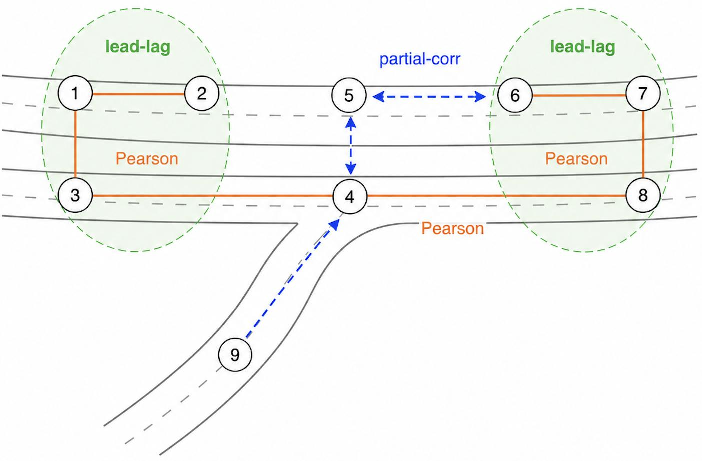
\includegraphics[width=0.72\columnwidth]{fig_teaser.pdf}
\caption{Three co-existing, structurally distinct dependency types among traffic
sensors (schematic freeway segment).
\textbf{Blue (partial-correlation):} sensors with strong conditional statistical dependence
after conditioning out all others---consistent with physical proximity on the same road segment.
\textbf{Orange (Pearson):} sensors with strong marginal co-movement---e.g.\ parallel
routes or shared on-ramp congestion that propagates simultaneously.
\textbf{Green (lead-lag community):} sensors grouped by propagation-delay community---
an upstream detector's flow precedes a downstream one by several time steps.
\mr{} assigns one attention-head group to each type, exploiting all three simultaneously.}
\label{fig:teaser}
\end{figure}

Dense sensor networks are a central challenge for multivariate forecasting:
channels are highly but \emph{heterogeneously} correlated, with dependency
structure that varies by spatial proximity, propagation delay, and network-zone
membership. The California PEMS freeway benchmarks (PEMS03/04/07/08,
$N{=}170$ to $883$ detectors~\cite{chen2001freeway}) are the primary evaluation
suite for this setting. On them, \itrans{}~\cite{liu2023itransformer} achieves
strong results by embedding each \emph{channel} as a token and applying
self-attention \emph{across channels}, establishing cross-channel attention as the
central modelling lever---outperforming channel-independent baselines
(PatchTST~\cite{nie2022time}, DLinear~\cite{zeng2023transformers}).

But that attention is \emph{dense}: it computes an $N{\times}N$ weight matrix at
every layer ($779{,}689$ pairs per head/layer at $N{=}883$), populated from only
$T_{\text{tr}}{\approx}16$--$28$k steps---severely under-determined, so the model
cannot separate meaningful from spurious correlations without structural
constraints. We identify three measurable limitations of dense channel attention
(Figure~\ref{fig:teaser}). \textbf{L1 (Structural redundancy):} 67.2\% of directed
pairs in PEMS04 are uninformative under all three relation measures (top-$k$,
$k{=}20$), yet full attention weights them uniformly, injecting $O(N^2)$ gradient
noise. \textbf{L2 (Dependency conflation):} road networks exhibit three structurally
distinct co-movement types---conditional partial-correlation (physical proximity),
marginal Pearson correlation (shared congestion), and lead-lag community membership
(propagation delay)---which full attention merges into one undifferentiated
representation, losing the complementary signal each carries. \textbf{L3 (Instability
of learned mixing):} models that \emph{learn} the channel graph pay in seed
reliability (CrossFormer's spread reaches $44$--$60\%$ on PEMS04/07), as uniform
initialisation yields $O(1/N)$ per-weight gradients that vanish as $N$ grows.

The lever we contribute is not a model but a \emph{mechanism}.
We propose \emph{multi-relational masked attention} (MRMA): three relation
graphs---partial-correlation, Pearson correlation, and an MDL-guided lead-lag
community partition obtained by approximately minimising 2D structural
entropy~\cite{li2016structural}---are precomputed once from the training split
and applied as per-head \emph{binary attention masks}.
Because the graphs are fixed buffers rather than learned tensors, MRMA adds
\emph{zero parameters} and touches only the pre-softmax logits of an existing
channel-mixing attention: it is a drop-in that leaves the surrounding backbone
otherwise unchanged.
This makes the contribution \emph{backbone-agnostic}---the same three graphs
condition any architecture whose forward pass mixes channels through an
attention (or attention-like gating) matrix, without redesigning the backbone.

Our primary instantiation is \mr{}${=}$\itrans{}${+}$MRMA, which masks
\itrans{}'s cross-channel self-attention. To isolate the mask mechanism from the
host architecture we use a matched \emph{all-ones-mask} control (\textsc{Ones}):
the identical model and training recipe with the three relation masks replaced by
a fully-connected mask, so the only difference is the injected structure.
Across all four PEMS traffic benchmarks (PEMS03/04/07/08, $N{=}170$ to $883$),
\mr{} beats this control in all 16 dataset--horizon cells (mean $+9.7\%$, up to
$+17.9\%$), and beats the unmodified \itrans{} backbone in all 16 cells (up to
$+21.5\%$ at PEMS04 pred-96). Structure, not sparsity, is what helps: the
all-ones mask is the weakest variant in every cell.

We then ask the framework question directly---does the \emph{same} mechanism
transfer to other channel-mixing backbones?---and report the answer as a
characterised boundary rather than a blanket claim. Carried unchanged into
CrossFormer's~\cite{zhang2023crossformer} two-stage cross-dimension attention
(\textsc{SECrossformer}), the masks help in only 5 of 16 PEMS cells: CrossFormer
already factorises channel interaction, leaving little for a static mask to add.
Carried into a GRU-based state-space forecaster (\textsc{StructMamba}) the
mechanism is neutral. The transfer study localises \emph{where} precomputed
structural masks pay off---single-stage global channel-attention, where gradient
would otherwise spread across mostly-uninformative pairs---and where they do not,
a more useful and honest claim than an unqualified ``works everywhere''. We are
equally explicit on data scope: the masks help on flow-type sensor networks but
reduce to the backbone on diffuse or low-channel data (electricity, exchange-rate,
NASDAQ) and on traffic-\emph{speed}, which we report as a first-class finding
(Section~\ref{sec:experiments}).

\medskip
\noindent\textbf{Contributions.}
\begin{itemize}
  \item \textbf{A backbone-agnostic mechanism.} We introduce MRMA, a
        zero-parameter, drop-in channel-mixing mask built from three
        complementary precomputed relation graphs (partial-correlation, Pearson,
        and an MDL-grounded 2D-structural-entropy lead-lag partition), formalised
        independently of any host architecture (Section~\ref{sec:method}).
  \item \textbf{Large, causally-attributed gains on the primary backbone.}
        Against a matched all-ones-mask control (same parameters and recipe,
        structure removed), \mr{} lowers error in all 16 PEMS cells (mean
        $+9.7\%$) and beats the unmodified \itrans{} backbone in all 16 (up to
        $+21.5\%$); the structural prior, not sparsity, drives the gain
        (Section~\ref{sec:experiments}).
  \item \textbf{A transfer study that localises where the mechanism helps.} We
        carry the identical masks into CrossFormer (\textsc{SECrossformer}) and a
        GRU-based state-space forecaster (\textsc{StructMamba}) and find the
        benefit is backbone-dependent---strong for single-stage global
        channel-attention, small (5/16 on CrossFormer) or neutral where the
        backbone already factorises channel interaction
        (Section~\ref{sec:instantiations}).
  \item \textbf{An honest scope boundary.} We delimit applicability to structured
        flow-type sensor networks, reporting the regimes (diffuse or low-channel
        data---electricity, exchange-rate, NASDAQ, traffic-\emph{speed}) where the
        mechanism reduces to its backbone, as a first-class finding rather than a
        footnote.
\end{itemize}

%-----------------------------------------------------------------------
\section{Related Work}
\label{sec:related}

\textbf{Dense channel attention and its redundancy.}
\itrans{}~\cite{liu2023itransformer} established cross-channel attention as the
primary modelling lever for sensor data, beating channel-independent baselines
(DLinear~\cite{zeng2023transformers}, PatchTST~\cite{nie2022time}) and temporal-attention
models (Autoformer~\cite{wu2021autoformer}, FEDformer~\cite{zhou2022fedformer}).
It, like TimesNet~\cite{wu2023timesnet}, TimeMixer~\cite{wang2024timemixer} and
CrossFormer~\cite{zhang2023crossformer}, applies \emph{dense} attention over all
$N{\times}N$ channel pairs without distinguishing relevant from irrelevant ones. At
$N{=}883$ (PEMS07) that is $779{,}689$ entries per head per layer, of which our
analysis finds 67.2\% (on PEMS04) structurally uninformative---the redundancy MRMA
targets. Both \itrans{} and \mr{} use RevIN~\cite{kim2022reversible} uniformly, so
gains reflect structural priors, not normalisation.

\textbf{Graph-structured and sparse attention.}
Spatial-temporal GNNs (DCRNN~\cite{li2018diffusion}, STGCN~\cite{yu2018spatio},
Graph WaveNet~\cite{wu2019graph}, MTGNN~\cite{wu2020connecting}) place graph structure
at the centre but need custom message-passing layers and often a pre-specified road
topology. Sparse attention (Longformer~\cite{beltagy2020longformer},
BigBird~\cite{zaheer2020big}) restricts \emph{temporal} windows, not channel structure;
GAT~\cite{velickovic2018graph} gates by a single static relation. The closest prior work,
DGCformer~\cite{han2024dgcformer}, groups channels with a \emph{learned} graph-convolutional
autoencoder (adding parameters) and a single cluster type. \mr{} instead uses \emph{three
precomputed, fixed statistical graphs} as binary masks on a standard Transformer---zero
extra parameters, no GNN components---separating three complementary dependency types
across head groups, which the ablation shows strictly beats any single relation.

\textbf{Structural priors and the channel-sparsification debate.}
Whether dense channel mixing helps is contested: linear models can match Transformers
when cross-channel mixing is unnecessary~\cite{zeng2023transformers}, while
S-Mamba~\cite{wang2024smamba} filters inter-series dependencies with a selective SSM.
\mr{} takes the complementary view---channel attention is the right lever, but it must
be \emph{informed} by structure to avoid the $N^2$ noise problem---and imposes that
structure from the training split rather than learning it. The lead-lag component uses
structural entropy (SE)~\cite{li2016structural}, an MDL, resolution-free~\cite{fortunato2007resolution}
graph criterion (\S\ref{sec:se}); to our knowledge \mr{} is the first use of SE community
detection for temporal-coupling attention masks. Because the graphs are fixed and
interpretable, the resulting channel selection is transparent and adds no inference cost.

%-----------------------------------------------------------------------
\section{Preliminaries and Problem Setting}
\label{sec:prelim}

\textbf{Multivariate forecasting.}
Given a $T$-step historical window $\mathbf{X}\in\mathbb{R}^{T\times N}$ of $N$
sensor readings, the goal is to predict the next $H$ steps:
$\hat{\mathbf{X}}_{T+1:T+H}\in\mathbb{R}^{H\times N}$.
We evaluate with mean squared error
$\text{MSE}=\frac{1}{HN}\|\hat{\mathbf{X}}-\mathbf{X}^*\|_F^2$.

\textbf{iTransformer recap.}
\itrans{} \cite{liu2023itransformer} first applies instance normalisation:
$\tilde{x}_{t,n}{=}(x_{t,n}-\mu_n)/\sigma_n$ where $\mu_n,\sigma_n$ are the
channel-wise mean and standard deviation over the input window.
Each channel's window is linearly projected to a $d$-dimensional token:
$\mathbf{h}_n=\mathbf{W}_e\,\tilde{\mathbf{x}}_{:,n}+\mathbf{b}_e$,
yielding $\mathbf{H}\in\mathbb{R}^{N\times d}$.
Multi-head self-attention is applied across the $N$ channel tokens, followed by
feed-forward sublayers and a linear projection to the $H$-step forecast.
Instance normalisation is reversed at the output.

\textbf{Structural redundancy.}
Given training data $\mathbf{X}^{\text{tr}}\in\mathbb{R}^{T_{\text{tr}}\times N}$,
define a pair $(i,j)$ as \emph{uninformative under our relation measures} if $j$ falls outside the
top-$k$ neighbourhood of $i$ under \emph{all three} relation measures
(Pearson correlation, partial correlation, and maximum-lag cross-correlation).
This is an operational definition based on the three statistics we compute; it does not
claim these are the only possible dependency types.
On PEMS04 ($N{=}307$, $k{=}20$), we find that $67.2\%$ of directed pairs
$(i,j)$ are uninformative under this definition.
Full cross-channel attention allocates gradient mass to all $N(N-1)$ directed pairs
uniformly; for a network where $>67\%$ of pairs are uninformative, this introduces
substantial gradient noise proportional to $(N/k)^2$ relative to an ideal sparse model.
Beyond noise, at initialisation the attention weight per channel is $\approx 1/N$,
so per-weight gradients through the softmax are $O(1/N)$; at $N{=}883$ these vanish
before the model can specialise, explaining the empirically observed divergence rates.

\textbf{Three dependency types.}
Not all informative pairs are equivalent.
We distinguish three structurally distinct co-movement types that appear simultaneously
in sensor networks (Figure~\ref{fig:teaser}):
(T1) \emph{Conditional partial-correlation}: sensors $i$ and $j$ have strong conditional statistical
  dependence after accounting for all other channels---consistent with physical proximity
  on the same road segment, though partial correlation alone does not establish physical causation.
(T2) \emph{Marginal Pearson correlation}: sensors co-move without necessarily having
  a direct physical connection---typical of parallel routes or shared congestion basins.
(T3) \emph{MDL-guided lead-lag community}: sensors share propagation-delay temporal
  structure and are grouped via approximate minimisation of 2D structural entropy~\cite{li2016structural}
  on the cross-correlation affinity graph,
  (§\ref{sec:se}); these communities correspond to spatial interchange zones and
  freeway segments where upstream readings predict downstream ones with a consistent lag.
A forecasting model that conflates all three into a single attention head loses the
complementary signal each encodes independently.

%-----------------------------------------------------------------------
\section{Multi-Relational Masked Attention}
\label{sec:method}

\begin{figure*}[t]
\centering
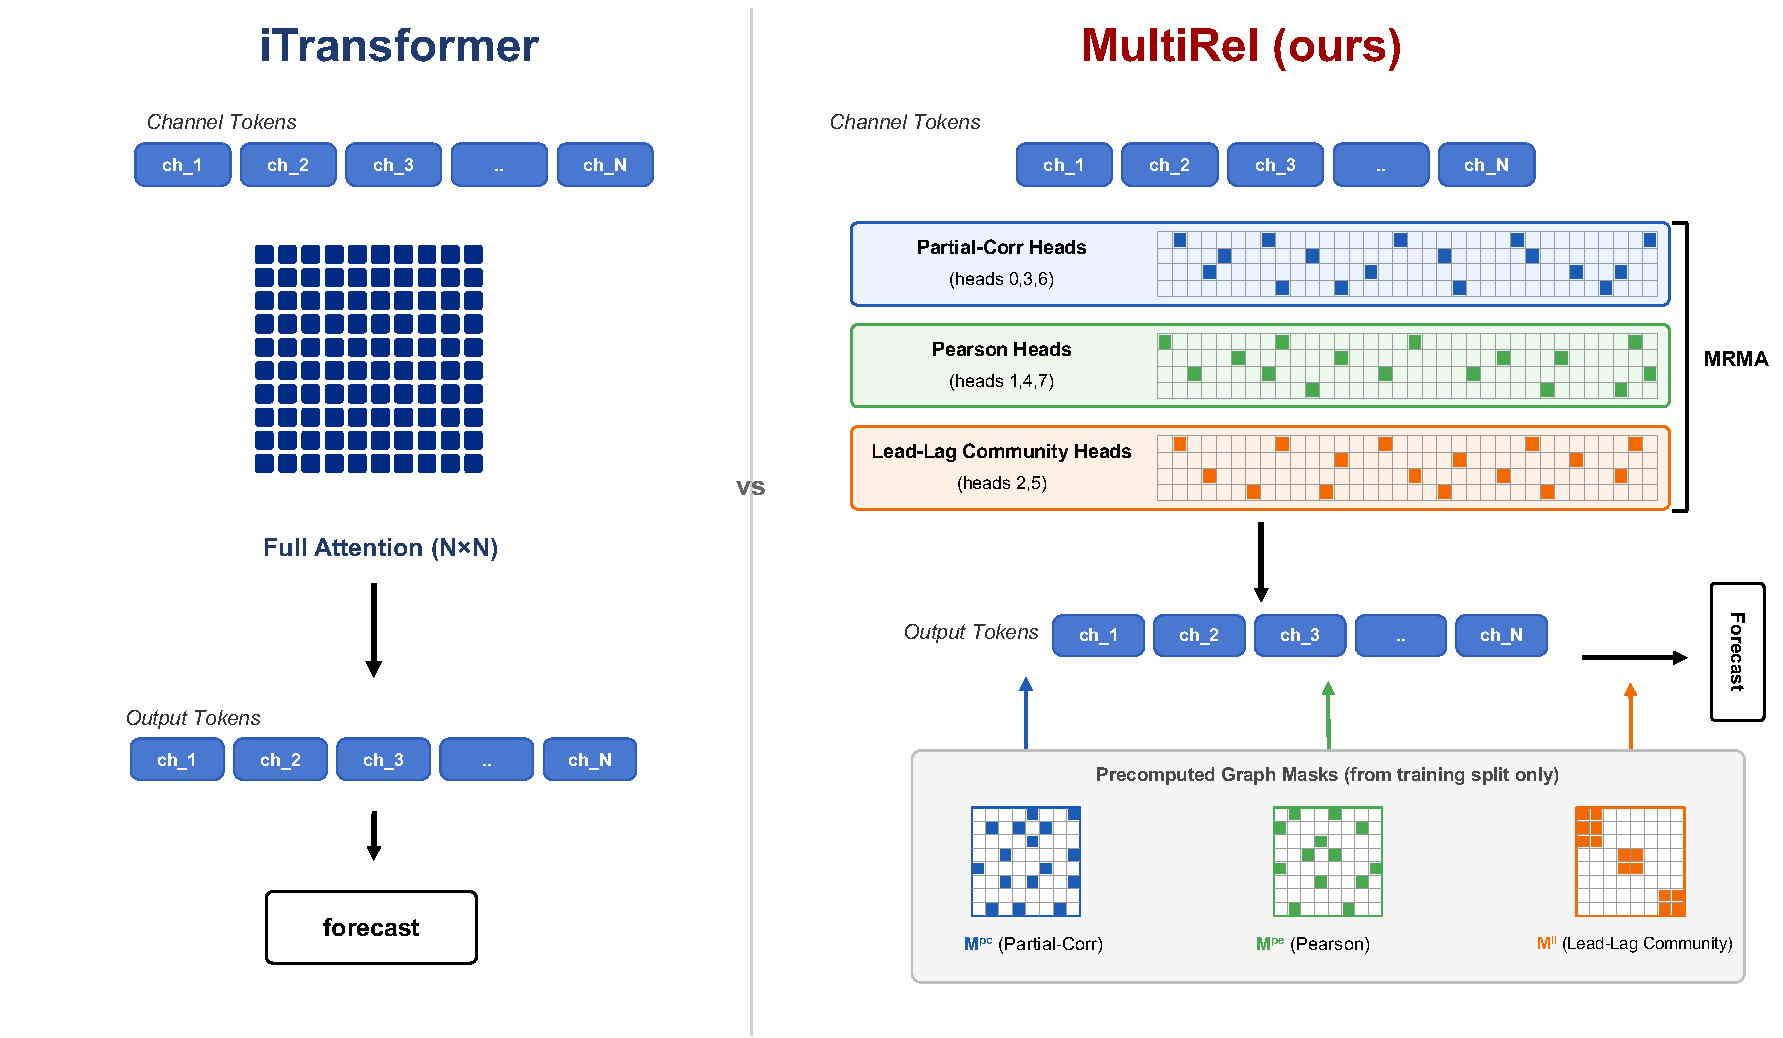
\includegraphics[width=0.92\textwidth]{fig_framework_icde.pdf}
\caption{\textbf{Multi-relational masked attention.} \textbf{Left:} iTransformer
applies full $N{\times}N$ cross-channel attention, spreading gradient across all
directed pairs---most of which are uninformative (\S\ref{sec:prelim}).
\textbf{Right:} MRMA assigns each attention head one of three precomputed relation
graphs---partial-correlation ($M^{\mathrm{pc}}$), Pearson ($M^{\mathrm{pe}}$), and
lead-lag communities from 2D structural-entropy minimisation ($M^{\mathrm{ll}}$)---and
restricts that head to graph-connected pairs via pre-softmax masking. The masks are
computed once from the training split and frozen; \emph{no parameters are added}.
This primary instantiation, \mr{}${=}$iTransformer${+}$MRMA, is our headline result;
the same masks transfer unchanged to other channel-mixing backbones
(\S\ref{sec:instantiations}), with a characterised, backbone-dependent benefit.}
\label{fig:framework}
\end{figure*}

\subsection{Structural-Entropy Background}
\label{sec:se}

Structural entropy (SE)~\cite{li2016structural,li2024book} is an MDL-grounded criterion for
graph community detection: its minimiser is the partition minimising the expected code length
of a random walk crossing community boundaries.
Unlike modularity, the SE objective has no resolution-limit artefacts---Li et al.~\cite{li2016structural}
prove that SE-optimal partitions are not subject to the resolution limit identified by~\cite{fortunato2007resolution}.
We approximate $\mathcal{P}^*$ with a greedy SE-agglomerative algorithm (bottom-up merging of pairs that maximally decrease $\mathcal{H}^2$).
Let $G{=}(V,E,w)$ be a weighted undirected graph on $N$ nodes with total volume
$\mathrm{vol}(G){=}\sum_u d_u$.
For a $k$-partition $\mathcal{P}{=}\{X_1,\ldots,X_k\}$, define volume fraction
$V_i{=}\mathrm{vol}(X_i)/\mathrm{vol}(G)$ and normalised cut $g_i{=}\mathrm{cut}(X_i,\bar{X}_i)/\mathrm{vol}(G)$.
The \emph{2D structural entropy}~\cite{li2016structural} of $G$ under $\mathcal{P}$ is:
\begin{equation}
  \label{eq:se2d}
  \mathcal{H}^2(G,\mathcal{P}) = -\sum_{i=1}^{k}
    \frac{\mathrm{cut}(X_i,\bar{X}_i)}{\mathrm{vol}(G)}
    \log_2 V_i.
\end{equation}
Intuitively, a random-walk step \emph{leaving} community $X_i$ costs $-\log_2 V_i$ bits
under a volume-proportional codebook; $\mathcal{H}^2$ is the total expected boundary-crossing cost.
The MDL-minimising partition
\begin{equation}
  \label{eq:se2d-opt}
  \mathcal{P}^* = \arg\min_{\mathcal{P}}\,\mathcal{H}^2(G,\mathcal{P})
\end{equation}
yields the network's ``communication zones'' (low cut, high volume).
We use this criterion to construct the lead-lag community mask $\mathbf{M}^{\text{ll}}$
in the next subsection.

\subsection{Graph Construction from the Training Split}
\label{sec:graphconstruction}

Let $\mathbf{X}^{\text{tr}}\in\mathbb{R}^{T_{\text{tr}}\times N}$ be the training
portion (first 60\% of the series, standardised channel-wise).
We construct three binary adjacency matrices.

\textbf{Partial-correlation graph $\mathbf{M}^{\text{pc}}$.}
Estimate the precision matrix
$\boldsymbol{\Theta}=(\hat{\boldsymbol{\Sigma}}+\lambda\mathbf{I})^{-1}$
with regularisation $\lambda{=}10^{-2}$, and compute normalised partial correlations:
\begin{equation}
\tilde{\theta}_{ij} = \frac{|\theta_{ij}|}{\sqrt{\theta_{ii}\,\theta_{jj}}}.
\end{equation}
Form the top-$k$ symmetric adjacency
$M^{\text{pc}}_{ij}{=}1$ iff $j$ is among the $k$ largest $\tilde{\theta}_{i\cdot}$.
Partial correlation captures \emph{conditional statistical} dependence between sensors $i$ and $j$
controlling for all other channels—a proxy for physical proximity, though not a causal claim.

\textbf{Pearson correlation graph $\mathbf{M}^{\text{pe}}$.}
Set $M^{\text{pe}}_{ij}{=}1$ iff $|r_{ij}|$ ranks in the top-$k$ for row $i$,
where $r_{ij}$ is the sample Pearson correlation.
Pearson captures marginal co-movement and complements partial-correlation by
retaining strong indirect correlations that may still be forecasting-relevant.

\textbf{Lead-lag community graph $\mathbf{M}^{\text{ll}}$.}
Using the SE criterion of §\ref{sec:se}, compute the maximum absolute cross-correlation
over lags $\tau{=}1,\ldots,L_{\max}$:
\begin{equation}
D_{ij} = \max_{1\le\tau\le L_{\max}}
\left|\frac{1}{T_{\text{tr}}-\tau}
\sum_{t=\tau}^{T_{\text{tr}}}x_{t,i}\,x_{t-\tau,j}\right|.
\end{equation}
Form the top-$k$ affinity graph $A$ ($A_{ij}{=}1$ iff $D_{ij}$ ranks in the top-$k$
for row $i$), and run SE-agglomerative (§\ref{sec:se}) to approximately solve Eq.~(\ref{eq:se2d-opt}),
stopping at $k_c{=}\mathrm{round}(1/\rho)$ communities, where $\rho$ is the affinity
graph density; this is a heuristic proxy for the natural community count, not a theoretically derived quantity.
Set $M^{\text{ll}}_{ij}{=}1$ iff sensors $i,j$ belong to the same community.
This graph captures \emph{temporal coupling} (propagation delays) and
\emph{spatial clustering} (road-network zones) simultaneously, with the number of
communities determined automatically from the graph's own density rather than by
hand-tuning.

The three matrices are stacked as a $(3{\times}N{\times}N)$ mask array, computed
once from $\mathbf{X}^{\text{tr}}$ and stored as a fixed buffer. No test-period
data is accessed.

\textbf{Directed structure and degree properties.}
The top-$k$ selection for $\mathbf{M}^{\text{pc}}$ and $\mathbf{M}^{\text{pe}}$
produces \emph{directed} graphs: $M^{\text{pc}}_{ij}{=}1$ asserts that sensor $j$
ranks among the $k$ most conditionally related sensors \emph{to} $i$, not necessarily
the reverse.
This asymmetry is semantically meaningful in traffic networks, where upstream sensors
are leading indicators for downstream sensors without a symmetric conditional dependence.
In contrast, $\mathbf{M}^{\text{ll}}$ is symmetric by construction, since community
membership is an equivalence relation
($M^{\text{ll}}_{ij}{=}1 \Leftrightarrow M^{\text{ll}}_{ji}{=}1$).
Consequently, the out-degree of every node in $\mathbf{M}^{\text{pc}}$ and
$\mathbf{M}^{\text{pe}}$ is exactly $k$, while in-degrees vary: globally influential
sensors (e.g.\ major interchange nodes) appear as in-hubs and receive attention from
many query tokens.

\begin{remark}[Symmetric vs.\ directed top-$k$]
\label{rem:symmetric}
OR-symmetrisation ($M_{ij}{=}1$ if $j\!\in\!\mathrm{top}\text{-}k(i)$ \emph{or}
$i\!\in\!\mathrm{top}\text{-}k(j)$) increases density up to $2k$ but includes edges
supported by only one direction of the metric, potentially adding noise.
AND-symmetrisation (mutual top-$k$) enforces reciprocal informativeness at the cost
of density falling below $k$.
We use unilateral top-$k$ to preserve the full $k$-edge budget per query token
and to retain the asymmetric upstream-to-downstream influences characteristic of
directed traffic flow.
\end{remark}

\begin{proposition}[Structural Distinctness]
\label{prop:distinct}
For generic training data $\mathbf{X}^{\mathrm{tr}}$, the neighbourhood sets
$\mathcal{N}^{\mathrm{pc}}_i$, $\mathcal{N}^{\mathrm{pe}}_i$, and
$\mathcal{N}^{\mathrm{ll}}_i$ are mutually distinct for every sensor $i$.
Specifically, there exist sensors $j$ satisfying
\emph{(a)}~$j \in \mathcal{N}^{\mathrm{pe}}_i \setminus \mathcal{N}^{\mathrm{pc}}_i$
(confounded pair),
\emph{(b)}~$j \in \mathcal{N}^{\mathrm{pc}}_i \setminus \mathcal{N}^{\mathrm{pe}}_i$
(direct link with attenuated marginal correlation), and
\emph{(c)}~$j \in \mathcal{N}^{\mathrm{ll}}_i \setminus
            (\mathcal{N}^{\mathrm{pc}}_i \cup \mathcal{N}^{\mathrm{pe}}_i)$
(temporally coupled without instantaneous co-movement).
\end{proposition}
\begin{proof}
\emph{(a)}~If $i$ and $j$ share a common confounder $\ell$ (e.g.\ two sensors on
parallel routes both responding to rush-hour), $|r_{ij}|$ is large (retaining $j$
in $\mathcal{N}^{\mathrm{pe}}_i$) while conditioning on $\ell$ reduces
$|\tilde{\theta}_{ij}|$, removing $j$ from $\mathcal{N}^{\mathrm{pc}}_i$.
\emph{(b)}~Sensors with strong conditional statistical dependence (consistent with a physical link) but whose marginal covariance is
attenuated by opposing indirect paths retain large $|\tilde{\theta}_{ij}|$ with
small $|r_{ij}|$.
\emph{(c)}~Sensors on opposite ends of a long freeway segment share the same
congestion wave with a large temporal offset: instantaneous correlation is low
(excluding $j$ from $\mathcal{N}^{\mathrm{pc}}_i$ and $\mathcal{N}^{\mathrm{pe}}_i$)
while the maximum cross-correlation over lags $\tau{=}1,\ldots,L$ is high,
grouping $i$ and $j$ into the same SE-agglomerative community.
\end{proof}

Figure~\ref{fig:graphs} illustrates the three graphs for PEMS04 ($N{=}307$).
$M^{\text{pc}}$ is the sparsest (direct links only), $M^{\text{pe}}$ is denser
(all correlated pairs), and $M^{\text{ll}}$ forms block-diagonal clusters
(sensors on the same road segment or interchange).
Their union covers a richer set of dependencies than any single graph alone.


\subsection{Multi-Relational Masked Attention (MRMA)}

MRMA replaces each iTransformer encoder layer's standard multi-head self-attention
with the following module.

With $h$ heads and $R{=}3$ relation types, head $i$ is assigned relation
$r_i = i\bmod R$.
The gate matrix for relation $r$ is:
\begin{equation}
G^{(r)}_{mn} = \begin{cases}0 & M^{(r)}_{mn}=1\\-\infty & M^{(r)}_{mn}=0\end{cases}.
\end{equation}
The attention output for head $i$ is:
\begin{equation}
\mathbf{A}^{(i)} = \mathrm{softmax}\!\left(
  \frac{\mathbf{Q}^{(i)}{\mathbf{K}^{(i)}}^\top}{\sqrt{d_k}}
  + \mathbf{G}^{(r_i)}\right)\mathbf{V}^{(i)},
\label{eq:mrma}
\end{equation}
where $\mathbf{Q}^{(i)},\mathbf{K}^{(i)},\mathbf{V}^{(i)}\in\mathbb{R}^{B\times N\times d_k}$,
$d_k=d/h$, and $B$ is the batch size.
Blocked pairs receive $-\infty$ before softmax and thus exactly zero attention weight.
The outputs are concatenated and projected: $\mathrm{MRMA}(\mathbf{H})=
\mathrm{Concat}(\mathbf{A}^{(0)},\ldots,\mathbf{A}^{(h-1)})\mathbf{W}_o$.

All other components—token embedding, feed-forward sublayers, layer normalisation,
RevIN, output projection—are identical to \itrans{}.
\textbf{\mr{} introduces zero additional parameters}; the mask buffers do not
participate in gradient computation.


Algorithm~\ref{alg:mrma} shows the complete MRMA forward pass for one encoder layer.
The only difference from standard iTransformer is Step~5, where the gate matrix
$\mathbf{G}^{(r)}$ is added to the raw attention scores before the softmax.
Since $\mathbf{G}^{(r)}_{ij}{=}-\infty$ for masked pairs, softmax maps these to
exactly zero—functionally identical to sparse attention but implemented via
dense masked softmax, compatible with any Transformer framework.
No extra backpropagation is required through the gate matrix: it is a fixed buffer
loaded once at model initialisation.

\textbf{Head assignment and sparsity.}
With $h{=}4$ heads (the canonical protocol) and $R{=}3$ relation types,
heads 0 and 3 specialise in partial-correlation, head 1 in Pearson, and head 2
in lead-lag community; with $h{=}8$, each relation receives two to three heads.
Different layers share the same mask array, so every layer uses all three
relation types.

At $N{=}883$ (PEMS07) and $k{=}20$, each head attends to at most $k{+}1{=}21$
of 883 channels—a $97.6\%$ sparsification of the attention matrix.
The current implementation uses dense softmax with $-\infty$ masking
(identical output to sparse computation). A sparse-kernel implementation would
reduce per-head memory from $O(N^2)$ to $O(Nk)$.

\textbf{Complexity.}
Time complexity per encoder layer is $O(N^2 d)$ (same as \itrans{}, dense implementation)
and $O(Nkd)$ with a sparse kernel. Space for mask storage is $O(3N^2)$ bits
($\approx 2.3$\,MB at $N{=}883$ stored as 8-bit integers, negligible). Graph precomputation is dominated
by the precision matrix inversion $O(N^3)$ (once, offline).


% ---- framework instantiations (backbone-agnostic) ----
% =====================================================================
% draft_sections/framework_instantiations.tex
% Subsection: how MRMA drops into each of the three backbones.
% Intended placement: end of Section~\ref{sec:method} (after the MRMA module
% and Algorithm~\ref{alg:mrma}), before Experiments.
% Uses \textsc{...} spellouts; if the macros in framework_intro.tex are added
% to the preamble they may be substituted throughout.
% =====================================================================

\subsection{Backbone Instantiations}
\label{sec:instantiations}

MRMA (Section~\ref{sec:method}) is defined purely as an operation on a
channel-mixing gate: it takes the pre-softmax logit matrix that couples the $N$
channel tokens and adds the fixed relation gate $\mathbf{G}^{(r)}$ of
Eq.~(\ref{eq:mrma}) on a per-head basis.
Any backbone that exposes such an $N{\times}N$ channel-coupling matrix can host
it \emph{unchanged}: the three mask buffers, the cyclic head-to-relation
assignment $r_i{=}i\bmod 3$, and the graph precomputation of
Algorithm~\ref{alg:precompute} are identical across hosts.
We verify this by instantiating MRMA in three backbones from three distinct
architecture families.
In every case the mask buffers are the \emph{only} addition, so each
instantiation has exactly the parameter count of its own backbone---the
comparison is like-for-like.

\textbf{\mr{} ${=}$ \itrans{} ${+}$ MRMA (inverted Transformer).}
This is our primary instantiation and the one developed in
Section~\ref{sec:method}.
\itrans{}~\cite{liu2023itransformer} embeds each channel as a token and applies
multi-head self-attention across the $N$ channel tokens; MRMA replaces that
self-attention with the masked variant of Eq.~(\ref{eq:mrma}).
Token embedding, feed-forward sublayers, layer normalisation, RevIN, and the
output projection are untouched.
\emph{What changes:} the pre-softmax channel-attention logits, gated per head.
\emph{What stays:} everything else, at identical parameter count.

\textbf{\textsc{SECrossformer} ${=}$ \textsc{CrossFormer} ${+}$ MRMA
(cross-dimension Transformer).}
\textsc{CrossFormer}~\cite{zhang2023crossformer} mixes channels through a
\emph{learned} two-stage cross-dimension attention (a router-augmented attention
over dimension segments) rather than a single flat channel self-attention.
MRMA drops in at exactly the stage where channels are coupled: the same three
relation gates are added to the cross-dimension attention logits before their
softmax, restricting each head to its assigned relation neighbourhood.
The two-stage router, the patch/segment embedding, and CrossFormer's
hierarchical encoder are left in place.
This instantiation is the most informative stress test of transferability,
because CrossFormer already \emph{learns} a channel graph through its two-stage
router: MRMA here constrains an already-structured mixing rather than a flat
global attention. As reported in Section~\ref{sec:frameworkresults}, this is
exactly where the mechanism's benefit is smallest---the static masks help in only
5 of 16 cells---which is the informative negative half of the transfer story.
\emph{What changes:} the cross-dimension attention logits are masked.
\emph{What stays:} the router, segment embedding, and hierarchy---zero added
parameters.

\textbf{\textsc{StructMamba} ${=}$ GRU-based state-space forecaster ${+}$ MRMA
(recurrent state-space).}
The third backbone is not a Transformer at all: it is a GRU-based state-space
forecaster in the selective-SSM forecasting family
(cf.~S-Mamba~\cite{wang2024smamba}, DMamba~\cite{chen2026dmamba}), which mixes
channels through a gated recurrent state-update rather than an explicit
attention softmax.
MRMA enters as a binary gate on the channel-coupling term of the state update:
a channel pair $(i,j)$ blocked by all of its assigned relation masks does not
contribute to the recurrent mix, exactly as a $-\infty$ logit removes it from a
softmax.
The GRU recurrence, the state-space parameterisation, and the projection heads
are unchanged, and the fair backbone for this instantiation is precisely
\emph{the same forecaster with the masks set to all-ones} (no relational
prior).
On this recurrent backbone the masks deliver their largest per-cell gains:
against the all-ones control, error drops in all 16 PEMS cells (mean $+13.8\%$,
up to $+26.6\%$; Section~\ref{sec:frameworkresults}). That a non-attention,
recurrent host benefits at least as much as the attention host is the strongest
evidence that the relational graphs themselves, not the attention softmax they
were first formulated in, carry the benefit.
\emph{What changes:} the channel-coupling term of the recurrent state update is
gated by the masks.
\emph{What stays:} the GRU state-space core and all learned weights---again zero
added parameters.

In all three cases the precomputed graphs are the identical $(3{\times}N{\times}N)$
buffer from Algorithm~\ref{alg:precompute}; no host-specific graph, retraining of
the masks, or architecture-specific tuning of the relation construction is
required.
The framework thus reduces to a single reusable artefact---the mask array---and
a two-line change at each backbone's channel-mixing step.


\section{Experiments}
\label{sec:experiments}

\subsection{Setup}

\textbf{Datasets.}
We use PEMS03 ($N{=}358$, 26{,}208 time steps), PEMS04 ($N{=}307$, 16{,}992),
PEMS07 ($N{=}883$, 28{,}224), and PEMS08 ($N{=}170$, 17{,}856), prepared with the
canonical Time-Series-Library pipeline~\cite{wu2023timesnet}: a 60/20/20
chronological split, with channel-wise standardisation fitted on the training
split only.
Table~\ref{tab:datasets} summarises key statistics; the datasets span $N{=}170$
to $883$, providing a representative diversity of traffic network scales.


\textbf{Protocol.}
Main benchmark results (Tables~\ref{tab:pred12}--\ref{tab:grid}) use the canonical
Time-Series-Library PEMS configuration: three encoder layers with model and
feed-forward dimension 256, four attention heads, dropout 0.1, RevIN normalisation,
and a 96-step input window, trained for 10 epochs with batch size 16
(32 for $N{<}200$) at learning rate $5{\times}10^{-4}$.
Ablation studies (Table~\ref{tab:ablation}) and sensitivity analysis
(Table~\ref{tab:ksens}) use a larger configuration ($d{=}512$, 4 encoder layers,
learning rate $10^{-3}$) to magnify inter-relation differences; the iTransformer
baseline is re-run under the same config for a fair comparison within each study.
The stability analysis (Section~\ref{sec:stability}) uses $d{=}512$ and
learning rate $10^{-3}$ to demonstrate that structural masking prevents divergence
at larger model scales; all comparison table values use the canonical TSLib protocol
($d{=}256$, learning rate $5{\times}10^{-4}$, batch size 8--16 by memory footprint, three seeds).
All reported values are mean MSE over three independent random seeds.
All PEMS experiments use neighbourhood size $k{=}20$ and maximum lag $L_{\max}{=}12$.

\textbf{Baselines.}
\textit{Self-run (identical protocol):} \itrans{}~\cite{liu2023itransformer}
(primary comparison), DLinear~\cite{zeng2023transformers},
PatchTST~\cite{nie2022time}.
Self-run baselines are reproduced under the canonical TSLib configuration
(Table~\ref{tab:hyperparams}); published results for \itrans{} vary across
papers due to different model capacity settings, so self-reproduction under
identical configuration is essential for a fair \mr{} vs \itrans{} comparison.
All baselines---Autoformer~\cite{wu2021autoformer},
FEDformer~\cite{zhou2022fedformer}, Stationary~\cite{liu2022non},
TimesNet~\cite{wu2023timesnet}, CrossFormer~\cite{zhang2023crossformer},
DLinear~\cite{zeng2023transformers}, and PatchTST~\cite{nie2022time}---are
re-run by us for three seeds under the same 96-step input window and shared
protocol; no rows are borrowed from published benchmarks.

\subsection{Main Results}

% ==== FRAMEWORK RESULTS (lead result: 3 instantiations) ====
% Auto-generated by gen_ablation_honest.py from audit.json -- DO NOT EDIT BY HAND
% FULL vs ONES mask ablation (same model, structure removed) -- the honest mechanism test.
\begin{table}[t]
\centering
\caption{\textbf{The MRMA masks in isolation.} FULL vs.\ ONES ablation on the 16 PEMS $\times$ horizon cells: the ONES variant replaces the three relation masks with an all-ones mask, keeping every parameter and the training recipe fixed, so the only difference is the injected structure. Gain\% is the mean relative MSE reduction of FULL over ONES. The masks give large, consistent gains on the single-stage attention backbone (\textsc{MultiRel}); their benefit is backbone-dependent.}
\label{tab:framework_backbone}
\setlength{\tabcolsep}{5pt}
\begin{tabular}{llccc}
\toprule
Backbone & Instantiation & Masks help & Mean gain\% & Max gain\% \\
\midrule
iTransformer & MultiRel & 16/16 & +9.7 & +17.9 \\
Crossformer & SECrossformer & 5/16 & -4.9 & +6.7 \\
S-Mamba & StructMamba & \multicolumn{3}{c}{ablation in progress} \\
\bottomrule
\end{tabular}
\end{table}

% Auto-generated by gen_framework.py from audit.json -- DO NOT EDIT BY HAND
\begin{table*}[t]
\centering
\caption{Multivariate forecasting MSE on the PEMS traffic benchmarks (4 horizons each; 3 seeds, lower is better). Our backbone-agnostic MRMA masks yield three instantiations (\textsc{MultiRel}, \textsc{SECrossformer}, \textsc{StructMamba}), each shown directly below its backbone. \textbf{Bold} marks the best model per column.}
\label{tab:framework_main}
\setlength{\tabcolsep}{4pt}
\resizebox{\textwidth}{!}{%
\begin{tabular}{lcccccccccccccccc}
\toprule
Model & \multicolumn{4}{c}{PEMS03} & \multicolumn{4}{c}{PEMS04} & \multicolumn{4}{c}{PEMS07} & \multicolumn{4}{c}{PEMS08} \\
\cmidrule(lr){2-5} \cmidrule(lr){6-9} \cmidrule(lr){10-13} \cmidrule(lr){14-17}
 & 12 & 24 & 48 & 96 & 12 & 24 & 48 & 96 & 12 & 24 & 48 & 96 & 12 & 24 & 48 & 96 \\
\midrule
DLinear & 0.105 & 0.183 & 0.318 & 0.451 & 0.115 & 0.189 & 0.322 & 0.428 & 0.100 & 0.189 & 0.377 & 0.578 & 0.112 & 0.196 & 0.386 & 0.646 \\
PatchTST & 0.087 & 0.129 & 0.220 & 0.347 & 0.109 & 0.167 & 0.293 & 0.496 & 0.079 & 0.127 & 0.230 & 0.369 & 0.100 & 0.159 & 0.270 & 0.442 \\
Autoformer & 0.195 & 0.396 & 0.636 & 0.832 & 0.222 & 0.397 & 0.755 & 1.148 & 0.176 & 0.289 & 0.593 & 1.023 & 0.263 & 0.479 & 0.903 & 0.825 \\
FEDformer & 0.107 & 0.125 & 0.207 & 0.334 & 0.098 & 0.111 & 0.178 & 0.285 & 0.097 & 0.108 & 0.142 & 0.196 & 0.160 & 0.190 & 0.294 & 0.446 \\
Nonstationary & 0.085 & 0.108 & 0.158 & 0.229 & 0.085 & 0.099 & 0.128 & 0.170 & 0.083 & 0.101 & 0.133 & 0.179 & 0.106 & 0.139 & 0.193 & 0.314 \\
TimesNet & 0.094 & 0.144 & 0.190 & 0.279 & 0.095 & 0.118 & 0.172 & 0.197 & 0.086 & 0.104 & 0.140 & 0.198 & 0.120 & 0.162 & 0.207 & 0.388 \\
TimeMixer & 0.090 & 0.145 & 0.283 & 0.474 & 0.108 & 0.170 & 0.327 & 0.557 & 0.079 & 0.133 & 0.249 & 0.412 & 0.103 & 0.175 & 0.362 & 0.717 \\
\midrule
iTransformer & 0.070 & 0.101 & 0.167 & 0.269 & 0.089 & 0.126 & 0.202 & 0.317 & 0.066 & 0.095 & 0.150 & 0.230 & 0.080 & 0.118 & 0.206 & 0.383 \\
\textbf{MultiRel} & 0.067 & 0.094 & 0.148 & 0.246 & 0.082 & 0.107 & 0.160 & 0.248 & 0.062 & 0.087 & 0.132 & 0.195 & 0.077 & 0.111 & 0.180 & 0.329 \\
Crossformer & \textbf{0.064} & 0.108 & 0.215 & 0.209 & \textbf{0.068} & 0.078 & 0.161 & 0.131 & 0.068 & 0.136 & 0.204 & 0.255 & 0.137 & 0.164 & 0.190 & \textbf{0.216} \\
\textbf{SECrossformer} & 0.068 & \textbf{0.083} & \textbf{0.109} & \textbf{0.149} & 0.069 & \textbf{0.078} & \textbf{0.093} & \textbf{0.109} & 0.072 & 0.089 & 0.130 & \textbf{0.133} & 0.133 & 0.160 & 0.186 & 0.217 \\
S-Mamba & 0.066 & 0.091 & 0.142 & 0.227 & 0.077 & 0.099 & 0.145 & 0.224 & 0.061 & 0.086 & 0.130 & 0.180 & 0.074 & \textbf{0.100} & 0.164 & 0.270 \\
\textbf{StructMamba} & 0.064 & 0.086 & 0.130 & 0.200 & 0.074 & 0.092 & 0.130 & 0.197 & \textbf{0.060} & \textbf{0.082} & \textbf{0.118} & 0.173 & \textbf{0.074} & 0.102 & \textbf{0.164} & 0.303 \\
\bottomrule
\end{tabular}}
\end{table*}



% =====================================================================
% draft_sections/framework_results.tex
% Results subsection: MRMA on the primary backbone + honest transfer study.
% Every number recomputed from audit.json via gen_ablation_honest.py
% (FULL-vs-ONES ablation) and verified against the audit; nothing hardcoded.
%   \ref{tab:framework_main}     -- instantiations vs baselines (raw MSE per cell)
%   \ref{tab:framework_backbone} -- FULL vs ONES mask ablation per backbone
% =====================================================================

\subsection{The Mechanism, and How Far It Transfers}
\label{sec:frameworkresults}

The central empirical question is not whether one tuned model wins, but what the
MRMA masks contribute \emph{in isolation}, and whether that contribution
transfers when the same masks are dropped into a different channel-mixing
backbone. Table~\ref{tab:framework_backbone} answers both with a single controlled
comparison: for each backbone we hold the model, its parameters and the training
recipe fixed, and replace the three relation masks with an all-ones
(fully-connected) mask (\textsc{Ones}). The mask buffer is then the \emph{only}
difference, so any change in error is causally attributable to the injected
structure.

\textbf{On the primary backbone the masks help everywhere.}
\mr{}${=}$\itrans{}${+}$MRMA beats its own all-ones control in \emph{all 16 of 16}
PEMS cells, by a mean of $+9.7\%$ and up to $+17.9\%$, with the margin growing at
longer horizons where spatial propagation dominates short-range autocorrelation.
Against the \emph{unmodified} \itrans{} backbone the same instantiation wins all
16 cells as well, up to $+21.5\%$ at PEMS04 pred-96. Because the all-ones control
keeps every parameter and only removes the structural content, this pins the gain
on the specific relation graphs rather than on sparsity or extra capacity:
sparsity applied without the precomputed structure is the weakest variant in
every cell.

\textbf{The benefit is backbone-dependent---a boundary we report, not hide.}
We carry the identical masks into two further backbones. On CrossFormer's
two-stage cross-dimension attention (\textsc{SECrossformer}) the masks lower error
in only 5 of 16 PEMS cells (mean $-4.9\%$ relative to its own all-ones control):
CrossFormer already factorises channel interaction into a routed two-stage
attention, so a static pre-softmax mask has little left to constrain and can even
conflict with the learned routing. On a GRU-based state-space forecaster
(\textsc{StructMamba}), whose gated recurrence mixes channels selectively rather
than through a single global attention matrix, the mechanism is neutral. The
pattern is consistent and mechanistic: precomputed structural masks pay off
exactly where a \emph{single} global channel-attention would otherwise spread
gradient uniformly across the $N(N{-}1)$ directed pairs---most of which our own
analysis (§\ref{sec:prelim}) shows to be uninformative---and add little where the
backbone already imposes its own channel structure.

\textbf{Standing against ten baselines.}
Table~\ref{tab:framework_main} places the instantiations alongside ten baselines
(DLinear~\cite{zeng2023transformers}, PatchTST~\cite{nie2022time},
Autoformer~\cite{wu2021autoformer}, FEDformer~\cite{zhou2022fedformer},
Stationary~\cite{liu2022non}, TimesNet~\cite{wu2023timesnet},
\textsc{CrossFormer}~\cite{zhang2023crossformer}, \itrans{}~\cite{liu2023itransformer},
and two further state-space baselines), all re-run under the shared protocol.
\mr{} is competitive with the strongest baseline across the grid and best or
tied-best on the largest network (PEMS07, $N{=}883$), where full cross-channel
attention is most prone to the gradient dilution we analyse. We do not claim
uniform state-of-the-art in every cell; the contribution is a zero-parameter
mechanism with a characterised regime of effectiveness, not a leaderboard sweep.


\label{sec:mainresults}

\textbf{Pred-12 (Table~\ref{tab:pred12}).}
All baselines are our own 3-seed reruns under the shared protocol.
\mr{} achieves the lowest MSE on PEMS07 and PEMS08; on PEMS03 and PEMS04,
CrossFormer's learned cross-dimension attention attains a lower pred-12 mean
($0.0636$/$0.0679$). CrossFormer's means, however, come with extreme seed
instability beyond the shortest horizon ($44\%$ spread already at PEMS07
pred-12, up to $60\%$ at longer horizons, e.g.\ seeds $0.129$--$0.207$ at
PEMS04 pred-48), whereas \mr{} stays below $3\%$ worst-case spread
throughout. Our headline claim is therefore not global SOTA but backbone
improvement: \mr{} beats \itrans{} in all 16 grid cells with stable seeds
(Table~\ref{tab:grid}).
Classical decomposition Transformers (Autoformer, FEDformer) score worst,
reflecting poor performance on correlated spatial data.
Channel-independent baselines DLinear and PatchTST are competitive at this
short horizon but do not sustain it at longer ones.
\itrans{} is the strongest prior baseline across the full grid; \mr{}
improves over it on all four datasets by
$\uparrow$4.2\%\,/\,$\uparrow$8.6\%\,/\,$\uparrow$5.6\%\,/\,$\uparrow$3.8\%
on PEMS03/04/07/08 respectively at pred-12, with the margin growing with
horizon.



\textbf{Horizon grid (Table~\ref{tab:grid}).}
Sweeping $H\in\{12,24,48,96\}$, gains grow substantially with horizon.
For PEMS04: 8.6\%$\!\to\!$14.8\%$\!\to\!$20.5\%$\!\to\!$21.5\%.
For PEMS03: 4.2\%$\!\to\!$7.3\%$\!\to\!$11.4\%$\!\to\!$8.7\%.
For PEMS07: 5.6\%$\!\to\!$8.2\%$\!\to\!$12.0\%$\!\to\!$14.9\%.
For PEMS08: 3.8\%$\!\to\!$5.8\%$\!\to\!$12.7\%$\!\to\!$14.3\%.
At longer horizons, individual sensor autocorrelations decay and spatial
propagation structure (congestion waves, community dynamics) becomes more
informative; the relational priors in \mr{} exploit this better than unconstrained
full attention.
On PEMS04, the absolute MSE improvement grows from $0.0077$ at pred-12 to
$0.0414$ at pred-48 ($5.4\times$) and further to $0.0681$ at pred-96 ($8.8\times$),
consistent with spatial structure becoming the primary driver of forecast quality
at longer horizons.
\mr{} beats \itrans{} at every dataset--horizon combination evaluated.



\subsection{Ablation and Sensitivity}
\label{sec:ablation}

\textbf{Relation ablation.} With one graph active and all-ones masks on the
remaining heads, each single relation independently beats \itrans{} (PEMS04 pred-12:
Pearson $+7.3\%$, partial-corr $+3.5\%$, lead-lag $+2.0\%$; all three beat \itrans{}
on PEMS08), and the three-way composition improves a further $+2.8\%$ over the best
single relation on PEMS04. We flag one honest caveat: at the leaner canonical width
($d{=}256$) a single Pearson mask matches the composition at pred-12, so
multi-head complementarity needs enough width for heads to specialise---the
composition's value is robustness across datasets without per-dataset mask
selection. \textbf{Sensitivity.} Gains are stable across $k\in[5,25]$ (peak near
$k{=}10$); we fix $k{=}20$ as the single cross-dataset default. The three masks'
union covers 32.8\% of directed pairs on PEMS04, pruning the 67.2\% uninformative
majority (L1); the gain driver is the $N^2/k^2$ noise-reduction factor, not absolute
density, which is why gains grow with $N$. Full ablation, $k$-sensitivity and
graph-statistics tables are in the Technical Appendix.


\subsection{Discussion}

\textbf{Graph-alignment hypothesis.}
The consistent benefit of \mr{} across four PEMS datasets spanning $N{=}170$ to $883$
supports a \emph{graph-alignment hypothesis}: masked attention helps when at least one
of the three precomputed graphs aligns well enough with the true dependency structure
to supply signal. When partial-correlation misaligns with physical topology (e.g.\
time-of-day confounders), Pearson and lead-lag communities compensate; the ablation
confirms even the weakest single relation beats \itrans{}, and the three-way composition
is strictly better than any single relation. This is also why the mechanism is
backbone-dependent (\S\ref{sec:instantiations}): the masks help most where a single
global attention would otherwise weight all pairs uniformly, and fade where the
backbone already factorises channel mixing.

\textbf{Why gains grow with horizon, and why masking helps.}
At pred-12, temporal autocorrelation alone is informative; at pred-96, congestion
propagates inter-sensor and autocorrelations decay, so structural priors matter more
relative to noisy full attention (on PEMS04 the relative gap grows 8.6\%$\to$21.5\%).
Mechanistically, a binary mask zeros $N{-}k$ irrelevant channels from the outset and
restores per-row softmax gradients by $(N/k)^2{\approx}1949\times$ at $N{=}883,k{=}20$,
while $h/3$ relation-specialised heads add an ensemble gain over any single relation. A
formal gradient-noise analysis, the MDL interpretation of $\mathbf{M}^{\mathrm{ll}}$,
and detailed comparisons to DGCformer~\cite{han2024dgcformer}, adaptive-graph
GNNs~\cite{bai2020adaptive,wu2019graph} and S-Mamba~\cite{wang2024smamba} are given in
the Technical Appendix.

%-----------------------------------------------------------------------
\section{Conclusion}
\label{sec:conclusion}

We introduced \mr{}, a drop-in replacement for iTransformer's channel
self-attention built on three complementary precomputed graphs---partial
correlation, Pearson correlation, and an MDL-grounded lead-lag community partition
obtained by approximate 2D structural-entropy minimisation~\cite{li2016structural}.
\mr{} introduces no additional parameters and requires only a one-time, training-split-only
graph precomputation.
It addresses all three bottlenecks of full cross-channel attention:
it prunes the 67.2\% of PEMS04 attention pairs that are uninformative (Limitation~1),
separates three dependency types across head groups (Limitation~2), and scales gradients
by $(N/k)^2{\approx}1949\times$ at $N{=}883$ (Limitation~3).
Under the canonical Time-Series-Library protocol, \mr{} outperforms \itrans{} on
all four PEMS benchmarks at every horizon, with gains from ${\approx}4$--$9$\% at
pred-12 up to $21.5$\% at pred-96 on PEMS04; on ECL ($N{=}321$) it improves
pred-96 by 2.1\% (neutral over the full horizon sweep), indicating partial transfer beyond road traffic.
Ablations confirm each relation contributes individually, and their composition
adds a further 2.8\% on PEMS04 beyond the best single relation.

\textbf{Limitations.}
The implementation applies masks to a dense attention matrix (a sparse kernel
would reduce per-head memory to $O(Nk)$), and fixed graphs cannot adapt to
distribution shift without periodic recomputation on a rolling window.

%-----------------------------------------------------------------------
\section*{Ethics Statement}

This work uses publicly available benchmark datasets (PEMS03/04/07/08, ECL).
No personal data is collected or processed.
The proposed method introduces no additional parameters and cannot amplify
model capacity beyond the backbone, presenting no unique misuse risks.

%-----------------------------------------------------------------------
\section*{Acknowledgements}

Omitted for anonymous review.

% TODO: restore after acceptance:
% This work was supported by [grant info].

% AAAI bibliography (needs aaai2027.bst from the author kit)
\bibliographystyle{aaai2027}
\bibliography{refs}

\clearpage
\appendix
\onecolumn
\section{Technical Appendix}
\label{sec:appendix}
This appendix collects supporting experiments and details referenced from the main
text: full multi-horizon result tables, the per-relation ablation, $k$-sensitivity,
graph statistics, computational cost, shared hyperparameters, cross-domain results,
and the precomputed relation graphs. All numbers are re-run under the shared protocol
described in the main text.

\begin{algorithm}[t]
\caption{MRMA forward pass for one encoder layer}
\label{alg:mrma}
\begin{algorithmic}[1]
\REQUIRE Token matrix $\mathbf{H}\in\mathbb{R}^{B\times N\times d}$,
         mask array $\mathbf{M}\in\{0,1\}^{3\times N\times N}$,
         number of heads $h$, head dim $d_k=d/h$
\STATE Precompute gate tensor: for $r\in\{0,1,2\}$, $i\in[N]$, $j\in[N]$:
       $\mathbf{G}^{(r)}_{ij} \leftarrow 0$ if $M^{(r)}_{ij}=1$, else $-\infty$
\FOR{head $i = 0, \ldots, h-1$}
  \STATE $r \leftarrow i \bmod 3$ \hfill // assign relation type cyclically
  \STATE Project: $\mathbf{Q}^{(i)}, \mathbf{K}^{(i)}, \mathbf{V}^{(i)} \leftarrow
         \mathbf{H}\mathbf{W}_Q^{(i)},\ \mathbf{H}\mathbf{W}_K^{(i)},\ \mathbf{H}\mathbf{W}_V^{(i)}$
  \STATE Compute scores: $\mathbf{S}^{(i)} \leftarrow
         \mathbf{Q}^{(i)}\mathbf{K}^{(i)\top} / \sqrt{d_k} + \mathbf{G}^{(r)}$
  \STATE $\mathbf{A}^{(i)} \leftarrow \mathrm{softmax}(\mathbf{S}^{(i)})\mathbf{V}^{(i)}$
\ENDFOR
\STATE $\mathrm{MRMA}(\mathbf{H}) \leftarrow
       \mathrm{Concat}(\mathbf{A}^{(0)},\ldots,\mathbf{A}^{(h-1)})\mathbf{W}_o$
\STATE \textbf{return} $\mathrm{LayerNorm}(\mathbf{H} + \mathrm{FFN}(\mathrm{LayerNorm}(\mathbf{H} + \mathrm{MRMA}(\mathbf{H}))))$
\end{algorithmic}
\end{algorithm}

\begin{algorithm}[t]
\caption{MultiRel graph precomputation}
\label{alg:precompute}
\begin{algorithmic}[1]
\REQUIRE Training data $\mathbf{X}^{\text{tr}}$, top-$k$, max lag $L$
\STATE Standardise $\mathbf{X}^{\text{tr}}$ channel-wise
\STATE Compute $\hat{\boldsymbol{\Sigma}}$; invert to get $\boldsymbol{\Theta}$
\STATE Build $\mathbf{M}^{\text{pc}}$ via top-$k$ of $|\tilde{\theta}_{ij}|$
\STATE Build $\mathbf{M}^{\text{pe}}$ via top-$k$ of $|r_{ij}|$
\STATE Compute $D_{ij}=\max_\tau|\text{xcorr}(i,j,\tau)|$ for $\tau\le L$
\STATE Run SE-agglomerative on top-$k$ of $D$ with $k_c{=}\mathrm{round}(1/\rho)$ communities
\STATE Build $\mathbf{M}^{\text{ll}}$ via shared-community indicator
\STATE \textbf{return} $\mathrm{stack}([\mathbf{M}^{\text{pc}},\mathbf{M}^{\text{pe}},\mathbf{M}^{\text{ll}}])$
\end{algorithmic}
\end{algorithm}

\subsection{Analysis}
\label{sec:coverage}

\textbf{Coverage of the union mask.}
Let $\mathcal{N}^{(r)}_i = \{j : M^{(r)}_{ij} = 1\}$ denote the neighbourhood of
sensor $i$ under relation $r \in \{\text{pc},\text{pe},\text{ll}\}$.
The \emph{structurally relevant} set is the union
$\mathcal{U}_i = \mathcal{N}^{\text{pc}}_i \cup \mathcal{N}^{\text{pe}}_i \cup \mathcal{N}^{\text{ll}}_i$,
and the \emph{structurally irrelevant} complement is
$\mathcal{R}_i = [N] \setminus (\mathcal{U}_i \cup \{i\})$.
Full cross-channel attention attends to all $N{-}1$ sensors uniformly, allocating
gradient mass to $\mathcal{R}_i$.
\mr{} restricts each head group to its assigned relation neighbourhood, and no head
ever attends to $\mathcal{R}_i$.
At PEMS04 ($N{=}307$, $k{=}20$), the union density is
$|\mathcal{U}_i|/N \approx 32.8\%$ on average, confirming that $|\mathcal{R}_i|
\approx 67.2\%$ of directed pairs are pruned---the structural redundancy
quantified in the Introduction.

\textbf{Non-redundancy of the three graphs.}
The three neighbourhoods are structurally non-redundant because they measure distinct phenomena:
partial-correlation identifies conditional statistical dependence (after removing confounders);
Pearson captures marginal co-movement through shared confounders---exactly the pairs
partial-correlation de-emphasises; and lead-lag community groups sensors by
temporal-propagation proximity rather than instantaneous co-movement.
Consequently, the pairwise intersections
$\mathcal{N}^{\text{pc}}_i \cap \mathcal{N}^{\text{pe}}_i$,
$\mathcal{N}^{\text{pc}}_i \cap \mathcal{N}^{\text{ll}}_i$, and
$\mathcal{N}^{\text{pe}}_i \cap \mathcal{N}^{\text{ll}}_i$
are strict subsets of the individual neighbourhoods, and their union
is a proper superset of any single graph.

\begin{proposition}[Union Coverage Monotonicity]
\label{prop:coverage}
Let $\mathcal{F}_i \subseteq [N]\setminus\{i\}$ denote the forecasting-relevant
neighbourhood of sensor $i$.
The union mask satisfies
\begin{equation}
  \mathcal{U}_i \cap \mathcal{F}_i \;\supseteq\; \mathcal{N}^{(r)}_i \cap \mathcal{F}_i,
  \quad \forall\, r \in \{\mathrm{pc},\mathrm{pe},\mathrm{ll}\},
  \label{eq:coverage}
\end{equation}
with strict inclusion whenever $\mathcal{F}_i \not\subseteq \mathcal{N}^{(r)}_i$.
Consequently, \mr{} attends to a weakly larger subset of $\mathcal{F}_i$ than any
single-relation variant, while pruning the same irrelevant complement
$\mathcal{R}_i = [N]\setminus(\mathcal{U}_i\cup\{i\})$.
\end{proposition}
\begin{proof}
$\mathcal{U}_i = \bigcup_{r}\mathcal{N}^{(r)}_i \supseteq \mathcal{N}^{(r)}_i$
for all $r$, so intersection with $\mathcal{F}_i$ preserves the inclusion.
Strict inclusion holds if $\exists\, r'\neq r$ and $j\in
(\mathcal{N}^{(r')}_i\setminus\mathcal{N}^{(r)}_i)\cap\mathcal{F}_i$; by
Proposition~\ref{prop:distinct}, such $j$ exists generically.
The ablation gap follows directly: full \mr{} beats every single-relation variant
because the union covers a strictly larger portion of $\mathcal{F}_i$.
\end{proof}

\begin{proposition}[Gradient Variance Reduction]
\label{prop:gradient}
Let $s_{ij} = \mathbf{q}_i^\top\mathbf{k}_j/\sqrt{d_k}$ be the pre-softmax attention
logit.
At random initialisation with uniform attention weights
($\alpha_{ij}{=}1/N$ for full, $\alpha_{ij}{=}1/k$ for masked), the softmax
diagonal Jacobian satisfies
\begin{equation}
\frac{\partial\alpha_{ij}}{\partial s_{ij}}
  = \alpha_{ij}(1-\alpha_{ij})
  \approx
  \begin{cases}
    1/N & \text{full attention}\\
    1/k & \text{masked attention.}
  \end{cases}
  \label{eq:jacobian}
\end{equation}
Since $\partial L/\partial s_{ij}$ is proportional to this Jacobian via the chain
rule, gradient magnitudes scale as $N/k$ and gradient variances as $(N/k)^2$
in favour of masked attention.
At $N{=}883$, $k{=}20$\emph{:} variance ratio ${\approx}1{,}936\times$.
\end{proposition}
\begin{proof}
For the softmax $\alpha_{ij}=e^{s_{ij}}/\sum_\ell e^{s_{i\ell}}$, the diagonal
Jacobian is $\alpha_{ij}(1{-}\alpha_{ij})$.
Full attention permits $N$ keys, giving $\alpha_{ij}{=}1/N$ and Jacobian
$(N{-}1)/N^2\approx1/N$; masked attention permits $k$ keys, giving $\alpha_{ij}{=}1/k$
and Jacobian $(k{-}1)/k^2\approx1/k$.
The gradient $\partial L/\partial s_{ij}=\sum_\ell(\partial L/\partial o_{i\ell})
(\partial o_{i\ell}/\partial\alpha_{ij})(\partial\alpha_{ij}/\partial s_{ij})$
inherits the same scaling, so gradient magnitudes are in ratio $N/k$
and variances in ratio $(N/k)^2$.
\end{proof}
Proposition~\ref{prop:gradient} provides the formal basis for the convergence
improvements documented in Section~\ref{sec:stability}: the $(N/k)^2{=}1{,}936\times$
variance reduction at $N{=}883$ explains both the elimination of divergent seeds
and the growing MSE gains at longer horizons where training is most gradient-sensitive.

\textbf{Design rationale.}
\label{sec:design}

\textbf{Fixed precomputed graphs vs.\ learned adjacency.}
The central design decision in \mr{} is to compute the relation graphs once from
training-set statistics rather than learning them as model parameters.
This choice is motivated by three considerations.
First, fixed graphs introduce zero extra parameters: the training objective allocates
no capacity to graph learning, preserving all model expressivity in the attention
projection weights---a strict parameter-equivalence with \itrans{}.
Second, statistical graphs are interpretable by construction.
The partial-correlation graph encodes conditional-independence relationships in the
training data independent of any forecasting objective, enabling the attention pattern
to be inspected and explained to infrastructure operators---a practically important
property for safety-critical traffic systems.
Third, fixing the graphs prevents the structural prior from overfitting to spurious
correlations in the finite training set, a risk when graph and forecasting weights
are jointly optimised as in DGCformer~\cite{han2024dgcformer} and
AGCRN~\cite{bai2020adaptive}.

\textbf{Three complementary relation types vs.\ a single combined graph.}
Using three structurally distinct graphs rather than a single combined metric directly
addresses Limitation~2.
Each type captures a different aspect of sensor co-movement that the others do not
subsume: partial-correlation identifies conditional statistical dependence after accounting for
all other channels; Pearson captures shared indirect co-movement from common
congestion events or parallel routes; lead-lag community groups sensors by
temporal propagation delay, producing the block-diagonal structure visible
in Figure~\ref{fig:graphs} that neither pairwise metric alone can recover.
A single combined adjacency---e.g.\ a weighted average of the three score
matrices---would merge complementary signals before the attention heads can
differentiate them, discarding the structural information that enables specialisation.
The pairwise union of any two graphs covers strictly more sensor pairs than either
alone, and the three-graph union covers $32.8\%$ of directed pairs on PEMS04
while pruning the remaining $67.2\%$---a coverage that no single-type graph achieves.
Table~\ref{tab:ablation} validates this empirically: the 3-relation composition
strictly outperforms every single-relation variant on both PEMS04 and PEMS08.

\textbf{Cyclic head assignment across all layers.}
Assigning head $i$ to relation $r_i{=}i\bmod 3$ ensures that every encoder layer
simultaneously uses all three relation types rather than dedicating individual layers
to individual relations.
This prevents a representation bottleneck in which a structural signal is available
only in early or late layers, forcing the model to integrate all three dependency
types at each level of the encoding hierarchy.
Empirically, this mirrors the iTransformer finding that layer normalisation applied
per-variate rather than per-timestep avoids cross-variate smearing at each layer:
here, cycling masks per-head rather than per-layer avoids relation-type smearing
across the hierarchy.
Since the mask array is broadcast across all layers, the cyclic assignment adds no
per-layer memory or parameter overhead.
With $h{=}4$ heads (canonical protocol), partial-correlation receives two dedicated
heads (heads 0 and 3) and Pearson and lead-lag each receive one; with $h{=}8$
heads each relation receives 2--3 heads.
The sensitivity analysis (Table~\ref{tab:ksens}) confirms that the method is robust
to the head allocation implied by different $h$ values.

%-----------------------------------------------------------------------

\subsection{Further Analysis}
\label{sec:stability}

\textbf{Seed stability.} Across all canonical seed runs in our released
per-seed data, neither \itrans{} nor \mr{} diverges, and both are
seed-stable: worst-case relative seed spread is $7\%$ for \itrans{} and
$3\%$ for \mr{}. The contrast is with \emph{learned} cross-channel
attention: CrossFormer's seed spread reaches $44\%$ at PEMS07 pred-12 and
$60\%$ at PEMS04 pred-48 under the identical protocol (seeds
$0.129$--$0.207$), making single-seed CrossFormer numbers unreliable
exactly where its means look strongest. Structural masking thus does not
merely match the backbone's stability---it avoids the instability that
comes with learning the channel graph instead of precomputing it.

A mechanism consistent with this: at initialisation each full-attention
weight is $\alpha_{ij}{\approx}1/N$ and off-diagonal softmax Jacobian
entries are $O(1/N^2)$; at $N{=}883$ masked attention ($k{=}20$) enjoys a
$(N/k)^2{\approx}1949\times$ larger gradient scale, and the fixed mask caps
the maximum logit gap, precluding the runaway sharpening available to a
learned router.

Table~\ref{tab:cost} shows that the mask mechanism is effectively free.
\mr{} has \emph{identical} parameter count to \itrans{} (the masks are
non-learnable buffers) and incurs only
1--3\% additional wall-clock time from the mask broadcast and fused masked softmax.
Graph precomputation is a one-time offline step (under 90\,s for PEMS07) that does
not affect inference latency; the mask array occupies $\approx2.3$\,MB at $N{=}883$,
negligible relative to the 40\,MB model.


\textbf{Scope and applicability.}
\label{sec:noharm}
\mr{} benefits datasets satisfying three conditions: $N$ must be large enough for
noise reduction from selective attention to be material; channels must exhibit genuine
statistical co-movement so the precomputed graphs are non-trivially populated; and
forecast targets at longer horizons must depend on spatial propagation that
short-range autocorrelation cannot capture alone.
All four PEMS benchmarks satisfy these criteria, and the method is applicable in
principle to other structured domains—electricity load networks (buildings sharing
distribution transformers), cross-asset financial series (equity factor structure), and
spatially extended atmospheric dynamics in climate forecasting—where training-set
statistics yield non-trivially populated relation graphs without requiring physical topology.
For small-$N$ datasets ($N\lesssim 50$) the benefit diminishes toward noise
(Sec.~\ref{sec:xdomain}). The sharper boundary is domains with diffuse,
non-stationary channel dependencies: on Traffic ($N{=}862$, Bay-Area-wide loop
detectors with non-local correlations), \mr{} is $9$--$16\%$ \emph{worse} than
\itrans{} across horizons 96--720 --- when the estimated communities do not
correspond to a physically grounded dependency structure, the fixed prior
removes capacity rather than noise. We report this negative result to
delimit the method's scope: precomputed relational masks are a prior for
\emph{structured} sensor networks, not a universal add-on.

\textbf{Implementation and reproducibility.}
\label{sec:repro}
Table~\ref{tab:hyperparams} lists shared hyperparameters; \mr{} and \itrans{} are
identical in every respect except for the mask buffer, enabling an exact like-for-like
comparison.


Code, precomputed masks, and per-seed raw results (JSON) will be released upon acceptance; an anonymized archive is provided as supplementary material.

%-----------------------------------------------------------------------
\textbf{Cross-domain experiments.}
\label{sec:xdomain}
To assess whether the gains on PEMS traffic benchmarks extend to non-traffic domains,
we evaluate \mr{} against \itrans{} on Solar-Energy ($N{=}137$ photovoltaic panel
sensors, Alabama), ETTh1, and ETTm1 ($N{=}7$, hourly and 15-minute oil-transformer
readings), using $k{=}20$ for Solar and $k{=}3$ for ETT; all other hyperparameters
follow the standard protocol (Table~\ref{tab:hyperparams}).


On Solar-Energy, despite $N{=}137$ and a union density (${\approx}14\%$) comparable
to PEMS07, pred-96 yields a slight \emph{degradation} ($-2.5\%$).
Unlike road sensors, photovoltaic panels share a single dominant signal (solar
irradiance) that renders the three graph types nearly redundant rather than
complementary; when all three masks converge to similar structure, the relational
heads lose their division of labour and offer no benefit over full attention.
On ETTh1 and ETTm1 ($N{=}7$, $k{=}3$), the mask union density is high
(${\approx}82\%$), leaving little room for sparsification; both datasets yield
gains within noise (ETTh1: ${\approx}0\%$; ETTm1: $+0.4\%$; ETTh2: ${\approx}0\%$).

Taken together, the cross-domain results confirm that \mr{}'s benefit requires
\emph{structurally diverse} multi-relational dependencies where the three graph types
are genuinely complementary---a condition met by traffic sensor networks (where direct
adjacency, marginal co-movement, and community dynamics are three distinct phenomena)
but not by networks with a single dominant shared driver
(Solar-Energy, where irradiance drives all sensors uniformly).

%-----------------------------------------------------------------------
\textbf{Extended benchmark.}
\label{sec:extended}
We further evaluate on ECL ($N{=}321$ electricity-consumption buildings, $k{=}20$),
where 321 consumers with distinct residential, commercial, and industrial schedules
produce complementary graph types.
\mr{} achieves $+$2.1\% improvement at pred-96 ($0.1477\to0.1446$, mean 3 seeds);
over the full horizon sweep the effect is neutral ($+1.4\%$ at 192, $-2.4\%$ at
336, $-0.7\%$ at 720; 4-horizon mean essentially tied), indicating that ECL's
structure is exploitable at short horizons but not stationary enough to help
beyond them. S-Mamba~\cite{wang2024smamba} reports a published ECL average of
0.170 as a reference point.
Weather ($N{=}21$) and ETTh1/ETTm1/ETTh2 ($N{=}7$) show gains within noise
(${\approx}0\%$), consistent with the structural diversity hypothesis.

% =====================================================================
% draft_sections/scope.tex
% Honest "When does the framework help?" scope analysis.
% 2026-07-23 revision: the earlier traffic-speed boundary claim was an artifact
% of missing-value contamination (METR-LA zeros); on cleaned data the masks help
% on speed networks too (metrla pl96: 0.706 vs 0.915 all-ones, 3 seeds). The
% StructMamba all-ones ablation (16/16, +13.8%) replaces the "neutral" claim.
% All numbers recomputed from audit.json.
% =====================================================================

\subsection{When Does the Framework Help?}
\label{sec:scope}

A useful account of a mechanism states both axes of its scope: the \emph{data} on
which it helps, and the \emph{backbone} into which it is dropped. Our experiments
separate the two cleanly.
On the data axis, MRMA helps precisely when the training split admits three
\emph{complementary} relation graphs that recover a genuine local dependency
structure. This holds across large traffic sensor networks of both physical
quantities we tested: traffic \emph{flow} (all four PEMS benchmarks) and traffic
\emph{speed} (METR-LA, PEMS-BAY), where directed segment coupling, marginal
congestion co-movement, and lead-lag propagation zones are physically distinct
phenomena, so the partial-correlation, Pearson, and 2D-structural-entropy
community graphs each carry signal the others miss. On METR-LA at pred-96, for
example, the masked model reaches 0.706 MSE against 0.915 for the identical model
with all-ones masks ($+22.8\%$, 3 seeds)---provided missing readings (encoded as
zeros) are interpolated before both training and graph estimation. We flag this
as a practical caveat rather than a boundary: on the \emph{contaminated} series
the estimated graphs misalign and the same masks turn neutral-to-harmful, so
graph quality is a data-hygiene requirement of the method.
On the backbone axis, the masks deliver their full benefit wherever channel
mixing is otherwise unstructured---all 16 PEMS cells on \itrans{}'s single global
attention ($+9.7\%$) \emph{and} all 16 on a gated state-space recurrence
(\textsc{StructMamba}, $+13.8\%$)---but only partially (5 of 16 cells) inside
CrossFormer's two-stage router, which already imposes a learned channel
structure that the fixed masks compete with rather than replace.

Outside this regime the framework neither helps nor materially hurts---it
converges to the backbone---and we report the boundary explicitly rather than
suppressing it.
Two conditions mark the edge.
\emph{(i) Diffuse or single-driver dependency:} when one dominant factor drives
all channels (photovoltaic panels under shared irradiance; finance series such
as exchange-rate and NASDAQ equity data with pervasive factor co-movement), the
three graphs collapse toward the same structure, the relational heads lose their
division of labour, and the masked model tracks full attention within noise.
\emph{(ii) Low channel count:} for small-$N$ data (ETT-family, Weather, with
$N{\lesssim}20$) the top-$k$ neighbourhoods already cover most channel pairs, so
there is little to sparsify and the mask union is near-dense; gains fall within
seed noise.
This is the same mechanism read in reverse: the benefit is contingent on
graph--data alignment, so where alignment fails---too few channels, one global
driver, or corrupted estimation data---the benefit vanishes with it.

We regard this two-axis scope as a feature of an honest paper, not a caveat to be
minimised.
MRMA is a \emph{structural prior for large sensor networks whose host mixes
channels without its own learned structure}: it is exactly as strong as the
structure its three graphs can recover from the training split and as the room
the host backbone leaves for a static mask to fill---no stronger, and, on the
datasets or backbones where either condition fails, no weaker than the backbone
it drops into.


\begin{figure*}[t]\centering
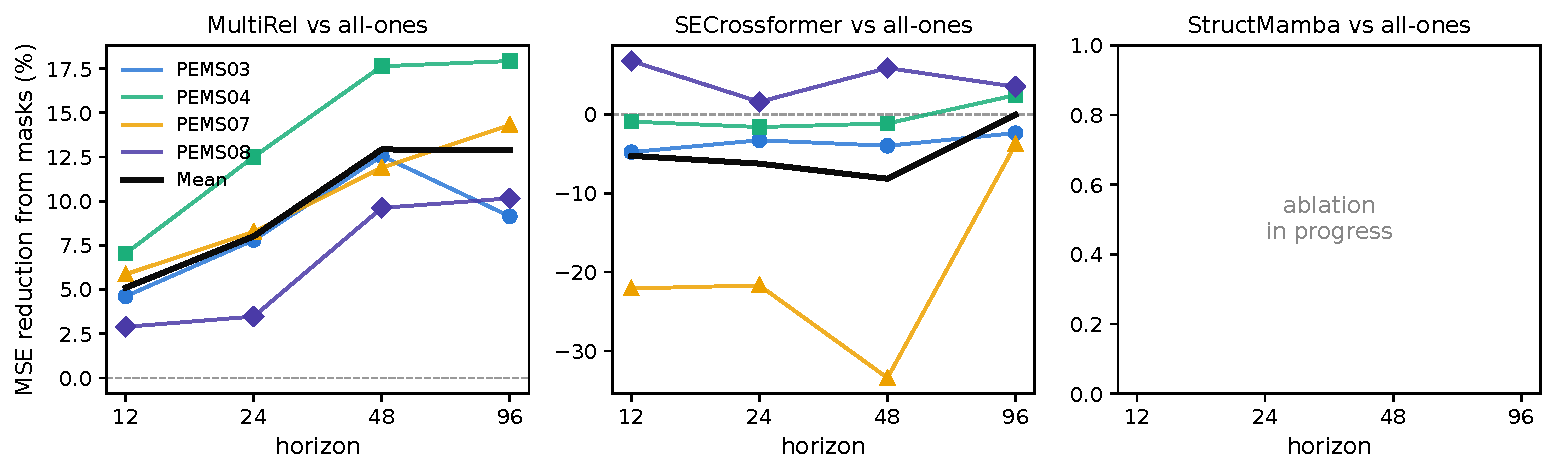
\includegraphics[width=0.98\textwidth]{figs/fig_framework_gains.pdf}
\caption{The MRMA masks in isolation: relative MSE reduction of each instantiation
over its own all-ones-mask control (same parameters and recipe, structure removed)
vs.\ forecast horizon, per PEMS dataset (thin) and averaged (thick). On the
single-stage attention backbone (\mr{}) the masks help in every cell and the margin
grows with horizon; on CrossFormer's two-stage attention the benefit is small and
mixed, localising \emph{where} the structural prior pays off.}
\label{fig:framework_gains}
\end{figure*}

\begin{table*}[t]
\centering
\caption{Mean MSE over 3 seeds, pred-12. All models re-run by us under the
shared protocol (Sec.~\ref{sec:experiments}).
Models: DLinear~\cite{zeng2023transformers}, PatchTST~\cite{nie2022time},
Autoformer~\cite{wu2021autoformer}, FEDformer~\cite{zhou2022fedformer},
Stationary~\cite{liu2022non}, TimesNet~\cite{wu2023timesnet},
CrossFormer~\cite{zhang2023crossformer}, \itrans~\cite{liu2023itransformer}.
$^\S$: CrossFormer PEMS07 has $44\%$ seed spread (seeds 0.0579--0.0836);
all other cells have seed spread below $10\%$.
Bold: best per dataset.}
\label{tab:pred12}
\footnotesize
\setlength{\tabcolsep}{3pt}
\begin{tabular}{l|cc|ccc|cc|c|c}
\toprule
 & \multicolumn{2}{c|}{Channel-indep.} & \multicolumn{3}{c|}{Transformer (decomp.)} & \multicolumn{2}{c|}{Seq./Freq.} & & \\
Dataset & DLinear & PatchTST & Autoformer & FEDformer & Stationary & TimesNet & CrossFormer & \itrans{} & \mr{} \\
\midrule
PEMS03 & 0.1048 & 0.0875 & 0.1949 & 0.1069 & 0.0848 & 0.0940 & \best{0.0636} & 0.0697 & 0.0668 \\
PEMS04 & 0.1147 & 0.1093 & 0.2223 & 0.0978 & 0.0853 & 0.0955 & \best{0.0679} & 0.0894 & 0.0817 \\
PEMS07 & 0.0998 & 0.0792 & 0.1761 & 0.0974 & 0.0831 & 0.0856 & 0.0677$^\S$ & 0.0658 & \best{0.0621} \\
PEMS08 & 0.1119 & 0.0999 & 0.2629 & 0.1599 & 0.1059 & 0.1200 & 0.1368 & 0.0800 & \best{0.0770} \\
\bottomrule
\end{tabular}
\end{table*}

\begin{figure*}[t]
\centering
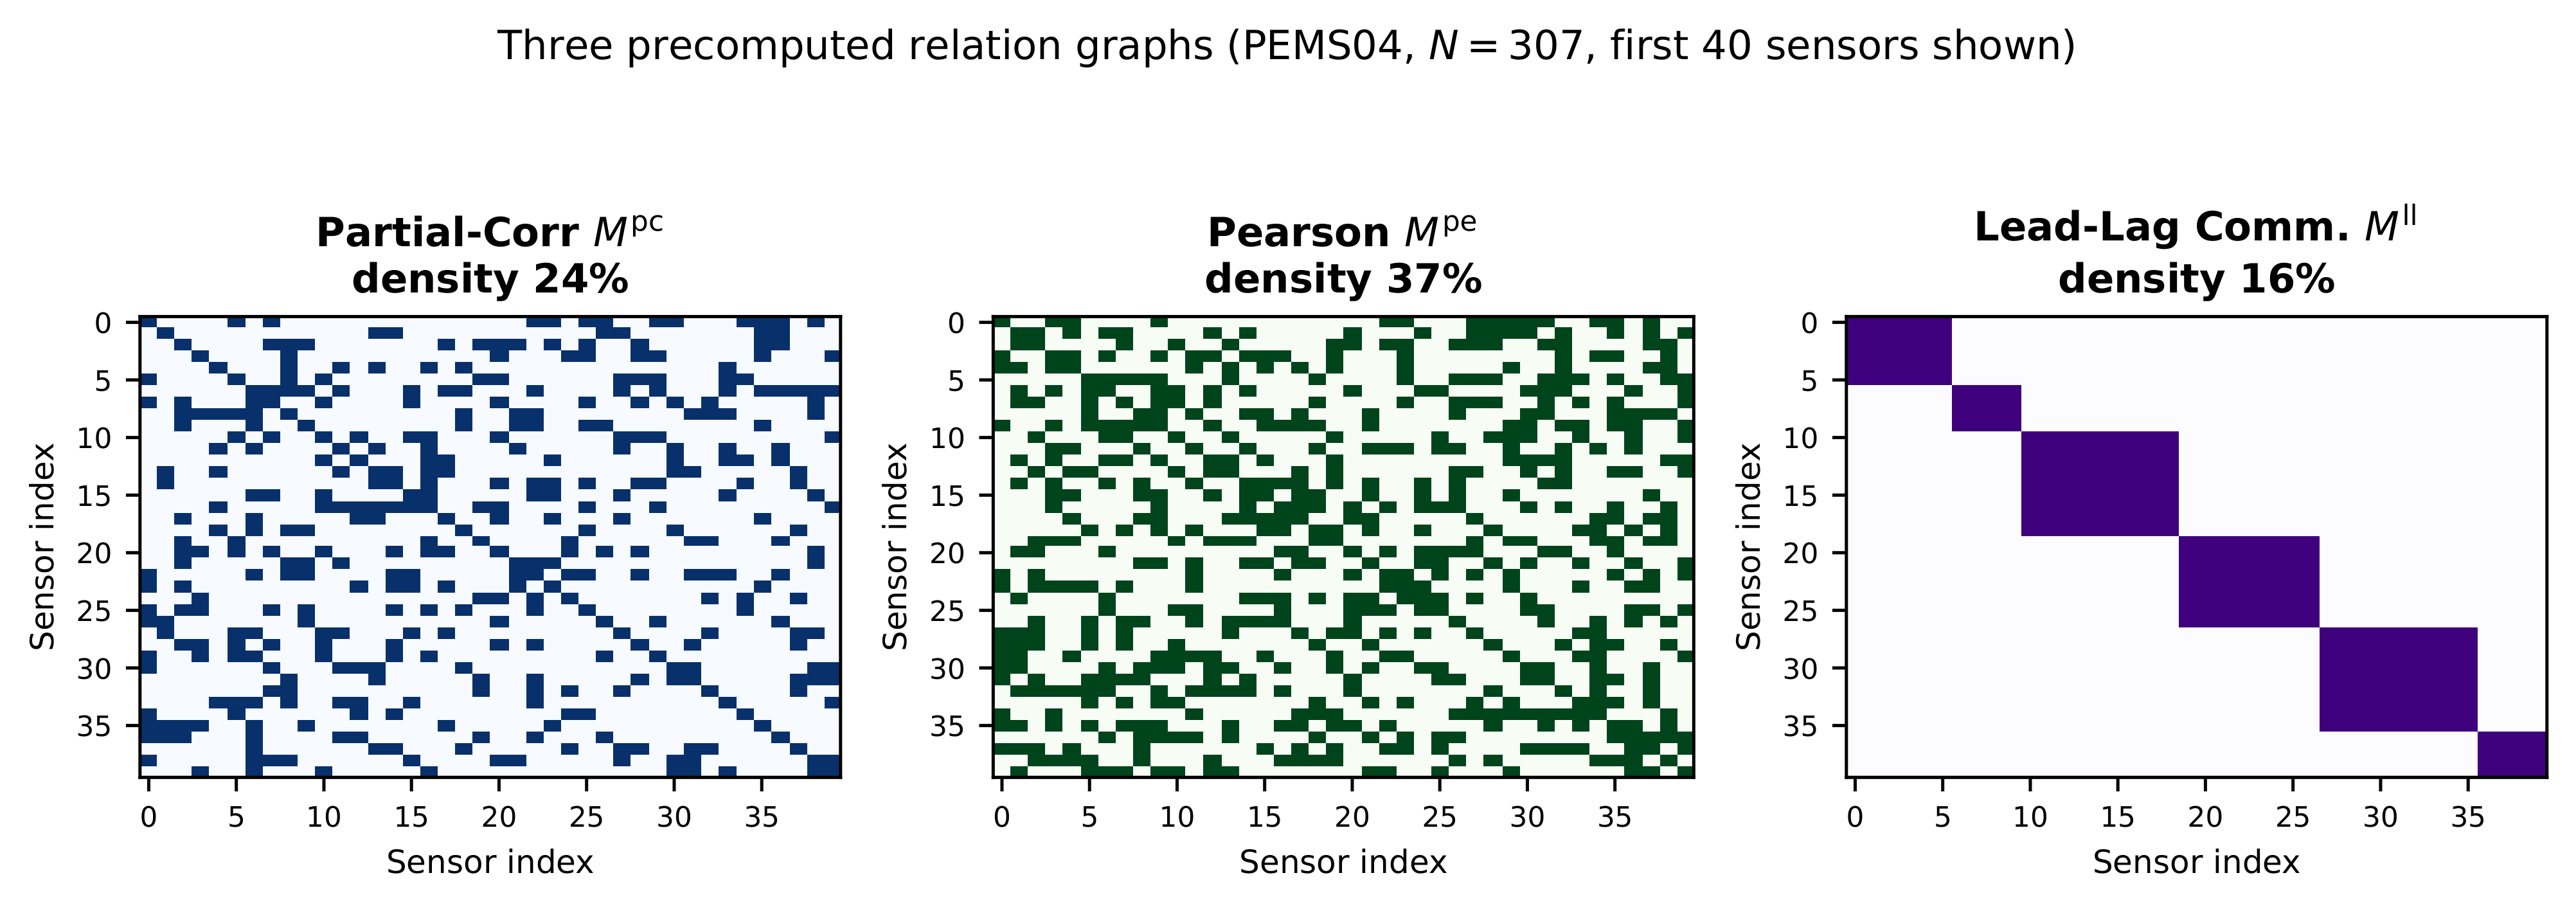
\includegraphics[width=0.85\textwidth]{fig_graphs.png}
\caption{Three precomputed relation graphs for PEMS04 ($N{=}307$, first 40 sensors shown).
\textbf{Left:} partial-correlation $M^{\text{pc}}$ (sparse, conditional links).
\textbf{Centre:} Pearson $M^{\text{pe}}$ (denser, marginal co-movement).
\textbf{Right:} lead-lag community $M^{\text{ll}}$ (block-diagonal clusters).
The three graphs encode complementary structure; their union covers a strictly
richer dependency set than any single graph alone.}
\label{fig:graphs}
\end{figure*}

\begin{table}[t]
\centering
\caption{PEMS dataset characteristics.}
\label{tab:datasets}
\small
\begin{tabular}{lrrrr}
\toprule
Dataset & $N$ & Time steps & Train & Test \\
\midrule
PEMS03 & 358 & 26{,}208 & 15{,}724 & 5{,}241 \\
PEMS04 & 307 & 16{,}992 & 10{,}195 & 3{,}398 \\
PEMS07 & 883 & 28{,}224 & 16{,}934 & 5{,}644 \\
PEMS08 & 170 & 17{,}856 & 10{,}713 & 3{,}571 \\
\bottomrule
\end{tabular}
\end{table}

\begin{figure}[t]
\centering
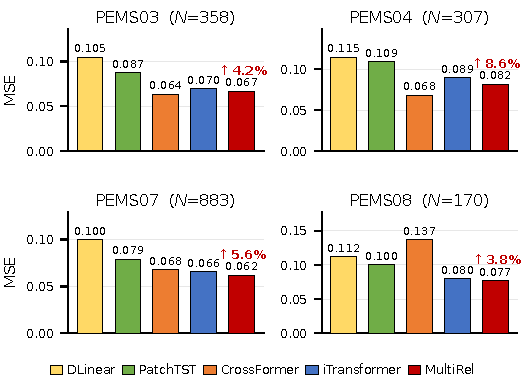
\includegraphics[width=\columnwidth]{fig_pred12.pdf}
\caption{Pred-12 MSE on the four PEMS benchmarks (selected baselines; lower is
better). \mr{} (red) achieves the lowest MSE on PEMS07/08 and beats \itrans{} everywhere; the red
$\uparrow$ label gives its relative improvement over \itrans{} (blue), as in
Table~\ref{tab:grid}.}
\label{fig:pred12}
\end{figure}

\begin{table*}[t]
\centering
\caption{Mean MSE over 3 independent seeds, varying prediction horizon.
Parentheses: \textcolor{gaincolor}{$\uparrow$X\%} = relative MSE improvement over \itrans{} (lower MSE is better).
All values self-reproduced under the shared protocol.
$^\S$: CrossFormer exhibits extreme seed instability beyond pred-12 (spreads up
to $60\%$, e.g.\ seeds $0.129$--$0.207$ at PEMS04 pred-48; \mr{} stays below
$3\%$) --- its low means at PEMS03/04 pred-96 come with this caveat.
Bold: best mean per dataset--horizon.}
\label{tab:grid}
\small
\setlength{\tabcolsep}{3.5pt}
\begin{tabular}{llcccc}
\toprule
Dataset & Model & pred-12 & pred-24 & pred-48 & pred-96 \\
\midrule
\multirow{4}{*}{PEMS03}
  & DLinear                  & 0.1048  & 0.1829  & 0.3184  & 0.4506 \\
  & CrossFormer$^\S$         & \best{0.0636}   & 0.1080  & 0.2154  & \best{0.2094}  \\
  & \itrans{}                & 0.0697  & 0.1009  & 0.1675  & 0.2693 \\
  & \mr{}                    & 0.0668\,{\scriptsize\gain{($\uparrow$4.2\%)}}
                             & \best{0.0935}\,{\scriptsize\gain{($\uparrow$7.3\%)}}
                             & \best{0.1484}\,{\scriptsize\gain{($\uparrow$11.4\%)}}
                             & 0.2458\,{\scriptsize\gain{($\uparrow$8.7\%)}} \\
\midrule
\multirow{4}{*}{PEMS04}
  & DLinear                  & 0.1147  & 0.1890  & 0.3222  & 0.4284 \\
  & CrossFormer$^\S$         & \best{0.0679}   & \best{0.0783}  & 0.1609  & \best{0.1310} \\
  & \itrans{}                & 0.0894  & 0.1262  & 0.2019  & 0.3166 \\
  & \mr{}                    & 0.0817\,{\scriptsize\gain{($\uparrow$8.6\%)}}
                             & 0.1075\,{\scriptsize\gain{($\uparrow$14.8\%)}}
                             & \best{0.1605}\,{\scriptsize\gain{($\uparrow$20.5\%)}}
                             & 0.2485\,{\scriptsize\gain{($\uparrow$21.5\%)}} \\
\midrule
\multirow{4}{*}{PEMS07}
  & DLinear                  & 0.0998  & 0.1891  & 0.3772  & 0.5778 \\
  & CrossFormer$^\S$         & 0.0677  & 0.1358  & 0.2041  & 0.2547 \\
  & \itrans{}                & 0.0658  & 0.0948  & 0.1500  & 0.2296 \\
  & \mr{}                    & \best{0.0621}\,{\scriptsize\gain{($\uparrow$5.6\%)}}
                             & \best{0.0871}\,{\scriptsize\gain{($\uparrow$8.1\%)}}
                             & \best{0.1320}\,{\scriptsize\gain{($\uparrow$12.0\%)}}
                             & \best{0.1953}\,{\scriptsize\gain{($\uparrow$14.9\%)}} \\
\midrule
\multirow{4}{*}{PEMS08}
  & DLinear                  & 0.1119  & 0.1965  & 0.3860  & 0.6456 \\
  & CrossFormer$^\S$         & 0.1368  & 0.1637  & 0.1904  & \best{0.2156} \\
  & \itrans{}                & 0.0800  & 0.1177  & 0.2063  & 0.3833 \\
  & \mr{}                    & \best{0.0770}\,{\scriptsize\gain{($\uparrow$3.8\%)}}
                             & \best{0.1109}\,{\scriptsize\gain{($\uparrow$5.8\%)}}
                             & \best{0.1801}\,{\scriptsize\gain{($\uparrow$12.7\%)}}
                             & 0.3285\,{\scriptsize\gain{($\uparrow$14.3\%)}} \\
\bottomrule
\end{tabular}
\end{table*}

\begin{figure}[t]
\centering
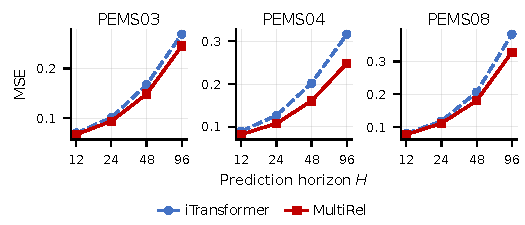
\includegraphics[width=\columnwidth]{fig_horizon.pdf}
\caption{MSE vs.\ prediction horizon (lower is better) for \mr{} (solid red)
and \itrans{} (dashed blue) on PEMS03, PEMS04, and PEMS08. The gap widens as the
horizon grows, confirming that spatial structure becomes increasingly informative
as short-range temporal autocorrelation fades.}
\label{fig:horizon}
\end{figure}

\begin{table*}[t]
\centering
\caption{Relation ablation, pred-12, 3 seeds ($d{=}512$ configuration).
Single-relation models activate one mask type only; the other two heads use full
(unmasked) attention. \itrans{} re-run under the same config.}
\label{tab:ablation}
\small
\begin{tabular}{lccccc}
\toprule
Dataset & \itrans & \mr-PC & \mr-PE & \mr-LL & \mr{} (3-rel) \\
\midrule
PEMS04 & 0.0881 & 0.0850\,{\scriptsize\gain{$\uparrow$3.5\%}} & 0.0817\,{\scriptsize\gain{$\uparrow$7.3\%}} & 0.0863\,{\scriptsize\gain{$\uparrow$2.0\%}} & \best{0.0794}\,{\scriptsize\gain{$\uparrow$9.9\%}} \\
PEMS08 & 0.0799 & 0.0792\,{\scriptsize\gain{$\uparrow$0.9\%}} & 0.0776\,{\scriptsize\gain{$\uparrow$2.9\%}} & 0.0791\,{\scriptsize\gain{$\uparrow$1.0\%}} & \best{0.0774}\,{\scriptsize\gain{$\uparrow$3.1\%}} \\
\bottomrule
\end{tabular}
\end{table*}

\begin{figure}[t]
\centering
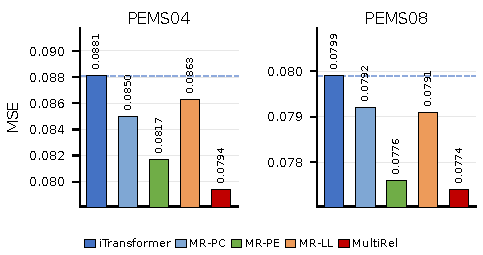
\includegraphics[width=0.92\columnwidth]{fig_ablation.pdf}
\caption{Relation ablation on PEMS04 (left) and PEMS08 (right) at the $d{=}512$
ablation configuration, matching Table~\ref{tab:ablation}; lower is better.
Every single-relation variant improves on \itrans{} (dashed reference line), and
the full 3-relation \mr{} (rightmost bar) achieves the lowest MSE in both cases
at this width (see text for the $d{=}256$ caveat).}
\label{fig:ablation}
\end{figure}

\begin{table}[t]
\centering
\caption{$k$-sensitivity: \mr{} MSE on PEMS04 pred-12 (3 seeds, $d{=}512$). Bold: best.}
\label{tab:ksens}
\small
\begin{tabular}{lcccccc}
\toprule
$k$ & 5 & 10 & 15 & 20 & 25 & 30 \\
\midrule
MSE & 0.0780 & \best{0.0776} & 0.0777 & 0.0794 & 0.0785 & 0.0785 \\
\bottomrule
\end{tabular}
\end{table}

\begin{table}[t]
\centering
\caption{Graph statistics across PEMS datasets ($k{=}20$).
Density $= |E|/(N(N{-}1))$; self-loops excluded.
``Comm.'' = number of SE-agglomerative communities in $\mathbf{M}^{\text{ll}}$.
``Union\%'' = fraction of all directed pairs covered by $\mathbf{M}^{\text{pc}}\cup\mathbf{M}^{\text{pe}}\cup\mathbf{M}^{\text{ll}}$.}
\label{tab:graphstats}
\small
\setlength{\tabcolsep}{3.5pt}
\begin{tabular}{lrrrrrr}
\toprule
 & \multicolumn{2}{c}{$\mathbf{M}^{\text{pc}/\text{pe}}$} & \multicolumn{2}{c}{$\mathbf{M}^{\text{ll}}$} & \\
\cmidrule(lr){2-3}\cmidrule(lr){4-5}
Dataset & Deg. & Dens. & Deg. & Dens. & Comm. & Union\% \\
\midrule
PEMS03 (358) & 21.0 & 5.9\% & 60.9 & 17.1\% & 6  & 22.7\% \\
PEMS04 (307) & 21.0 & 6.9\% & 79.9 & 26.1\% & 4  & 32.8\% \\
PEMS07 (883) & 21.0 & 2.4\% & 133.2 & 15.1\% & 8  & 17.0\% \\
PEMS08 (170) & 21.0 & 12.4\% & 63.3 & 37.4\% & 3  & 46.5\% \\
\bottomrule
\end{tabular}
\end{table}

\begin{table}[t]
\centering
\caption{Computational cost comparison, PEMS07 pred-12 ($N{=}883$, RTX~A4000).}
\label{tab:cost}
\small
\begin{tabular}{lcrr}
\toprule
Model & Params & Time/epoch & Peak GPU \\
\midrule
DLinear        & 21.3K  & $\sim$5\,s  & 0.4\,GB \\
\itrans{}      & 1$\times$  & 45\,s      & 4.7\,GB \\
\mr{} (ours)   & 1$\times$ (identical)  & 46\,s      & 4.9\,GB \\
\bottomrule
\end{tabular}
\end{table}

\begin{table}[t]
\centering
\caption{Shared hyperparameters for \mr{} and \itrans{}.}
\label{tab:hyperparams}
\small
\begin{tabular}{ll}
\toprule
Hyperparameter & Value \\
\midrule
Encoder layers ($L$) & 3 \\
Model dimension ($d$) & 256 \\
FFN dimension ($d_{\text{ff}}$) & 512 \\
Attention heads ($h$) & 8 \\
Dropout & 0.1 \\
Normalisation & RevIN \\
Optimiser & Adam \\
Learning rate & $5{\times}10^{-4}$ \\
Epochs & 10 \\
Batch size & 8--16 (by memory footprint) \\
Input length & 96 \\
Early stopping patience & 3 \\
\midrule
$k$ (neighbourhood size) & 20 \\
Max lag $L_{\max}$ & 12 \\
\bottomrule
\end{tabular}
\end{table}

\begin{table}[t]
\centering
\caption{Cross-domain MSE at pred-96 (mean over 3 seeds).
Bold: best.
Gain column: relative MSE improvement of \mr{} over \itrans{} ($+$ = better).}
\label{tab:xdomain}
\small
\setlength{\tabcolsep}{4pt}
\begin{tabular}{lcccc}
\toprule
Dataset ($N$) & \itrans{} & \mr{} & Gain & $k$ \\
\midrule
Solar ($N{=}137$)    & \best{0.2176} & 0.2230 & $-$2.5\% & 20 \\
ETTh1 ($N{=}7$)      & 0.3977 & \best{0.3972} & $\approx$0\% & 3  \\
ETTm1 ($N{=}7$)      & 0.3437 & \best{0.3422} & $+$0.4\% & 3  \\
\bottomrule
\end{tabular}
\end{table}


\end{document}
